%!TEX root = ../thesis.tex
\chapter{Numerical investigations\label{sec: numerics}}
We have now established multiple methods for approximating fluid queues which suitable for approximating the performance measures for fluid-fluid queues derived in \cite{bo2014}. In this chapter we numerically investigate various aspects of the approximation schemes. Throughout, we compare the QBD-RAP scheme (from Chapters~\ref{sec: conv} and \ref{sec: construction and modelling}), the discontinuous Galerkin method (without limiters or filtering of the solution) (as decribed in Chapter~\ref{ch:galerkin}), and the spatially-coherent uniformisation as described in \cite{bo2013} (which we will refer to a just the \emph{uniformisation scheme}). Recall that the uniformisation scheme is equivalent to a discontinuous Galerkin scheme with a constant basis function in each cell, which is also equivalent to the finite-volume method with an upwind flux. Like the QBD-RAP scheme, due to its stochastic interpretation, the uniformisation scheme is positivity preserving. 


Where appropriate, we also compare the above methods with the discontinuous Galerkin method with a slope-limiter implemented, which avoids oscillations and negative solutions. However, recall that, in the context of approximating operators of fluid-fluid queues with these schemes, slope-limiting is not possible, and even when slope limiting is possible, the resultant approximation is at best linear around discontinuities. 

The main focus of our numerical experiments is on the convergence properties as the number of basis functions is increased. For discontinuous Galerkin method, this means increasing the number of basis functions used to approximate the solution within each cell. For the QBD-RAP scheme, this means increasing the order of the CME distribution used to construct the scheme. For the uniformisation scheme, this means dividing each cell into smaller sub-cells over which we approximate the solution. As such, each approximation scheme leads to approximations which are matrices of the same size (although not necessarily the same number of non-zero components). For example, if we use 3 basis functions in the discontinuous Galerkin method, we approximate the solution by a quadratic on each cell; the comparable QBD-RAP scheme is to use a CME of order 3; and the comparable uniformisation scheme is to divide each cell into 3 sub-cells of width \(\Delta/3\). 

To keep the content of this chapter contained, we do not investigate the performance of the schemes as the cell sizes are decreased, other than for the uniformisation scheme. As such, for each numerical experiment, we keep the cell size fixed. As part of deriving a discontinuous Galerkin scheme, one needs to choose the \emph{numerical flux} which is used to approximate the transition of density from one cell to the next and link all the cells together. We investigate schemes with an upwind flux only.
We do not investigate the stability of the schemes with respect to the step-size of the time-integration or time-integration scheme (where required). Instead, we fix the time-integration step size for each numerical experiment at a suitably small value so as to obey a certain stability criterion (a CFL-like condition, REFs, appendix?). For schemes which require us to integrate over time we always implement the strong stability preserving Runge-Kutta method of order 4 with 5 stages (see appendix and REF). This scheme claims to introduce no more oscillations into the solution as we integrate over time (REFs). Where a slope limiter is implemented, we always implement the \emph{Generalised MUSCL} limiter (REF and Appendix). We do not investigate filtering for the DG scheme (REFs).

The performance of the discontinuous Galerkin method has been well-studied (REFs), and it is well-known that the discontinuous Galerkin method performs remarkably well on problems with smooth solutions (REF). Here, we mostly focus on investigating the numerical performance of the methods on problems with non-smooth solutions, the purpose of this is to emphasise the positivity-preserving properties of the QBD-RAP method. In the stochastic modelling community it is very common to have problems with discontinuous solutions, such as a non-smooth initial conditions (REFs). Even if a fluid-queue is initialised with a smooth initial density, the boundary dynamics may induce transient discontinuities into the problem. There is a very specific set of conditions on the initial density and point masses which must hold for the distribution of the fluid queue to remain smooth as it evolves over time (REFs).Limiting distributions of fluid queues are smooth, however. Further, it is possible that discontinuities are present in the performance measures of fluid-fluid queues. 

As we shall see, if the solution is smooth, then the Galerkin method is highly-effective and displays rapid convergence to the solution as the number polynomial basis functions is increased. However, when the solution is non-smooth oscillations and negative approximations may occur when using the discontinuous Galerkin method, leading to non-sensical solutions. In these cases, the QBD-RAP approximation performs relatively well compared to the other positivity preserving schemes investigated.

% THE STRUCTURE OF THE CHAPTER IS AS FOLLOWS. 

% 1. FUNCTION APPROX./RECONSTRUCTION

% 2. 1d wave eqn

% 3. STATIONARY DISTRIBUTIONS
	% i. SIMPLER
	% ii. MORE COMPLEX
	
% 4. TRANSIENT DISTRIBUTIONS 
	% i. SIMPLER
	% ii. MORE COMPLEX

% 5. HITTING TIMES 
	% i. SIMPLER
	% ii. MORE COMPLEX

% 6. FLUID-FLUID QUEUES

% 7. CONCLUDING REMARKS 

\section{Function approximation/reconstruction}
We start our investigation by looking at how well the methods perform at approximating an initial condition. For the discontinuous Galerkin method, this means projecting the solution on to the set of polynomial functions which define the scheme, then reconstructing the solution. For the spatially-coherent uniformisation scheme, this means looking at the sub-cell averages. For the QBD-RAP scheme, this means computing the initial vector for the approximation, then reconstructing the solutions as described in Section~\ref{sec: closing}. First we investigate three closing vectors we can use for the reconstruction for the QBD-RAP, from which we find that the closing operator in (\ref{eqn:5462}) performs reasonably compared to the others, and we are able to theoretically prove that it converges. Therefore we use this reconstruction method throughout the rest of the chapter.

For this section we consider approximating the initial condition over a single cell of width \(\Delta = 1\). To numerically evaluate integrals arising in the approximation step (inner products and cell averages) we use a simple trapezoidal rule with 10,001 function evaluations. Similarly, we use 10,001 function evaluations to approximate \(L^2\) norms, and also as a finite set of points over which to compute the KS statistics. 

First we briefly investigate the possible choices of closing operators as introduced in Section~\ref{sec: closing}. 

\subsection{QBD-RAP closing operators}
The three closing operators we investigate are the following. The unnormalised closing vector in Equation~(\ref{eqn: alal}). A normalised version of the closing operator in Equation~(\ref{eqn:546}), with the normalised version given by (\ref{eqn: nonlin}). We refer to the closing vector in (\ref{eqn: nonlin}) as the \emph{naive normalised} closing vector. Technically we have not yet proved that the \emph{naive normalised} closing vector leads to a convergent approximation scheme, though it clearly appears to converge. The third closing vector we investigate is that in Equation~(\ref{eqn:5462}). 

\begin{example}First consider approximating the initial condition with density function \(1(x<0.5)\). In the left-hand side of Figure~\ref{fig: fun 2 ks error qbdrap closing vecs} we plot the Kolmogorov-Smirnov error between the true CDF and the CDF constructed via the QBD-RAP approximation. Interestingly, in this case, the unnormalised error outperforms the other two reconstructions at low orders. It just so happens that, in this case, the error due to truncation of the unnormalised reconstruction destructively interferes with other errors in the reconstruction to cause the error to be lower at low orders for the unnormalised scheme. Figure~\ref{fig: fun 2 ks error qbdrap closing vecs} also shows that the naive normalised and normalised reconstructions perform very similarly -- this is the case throughout much of this subsection. The difference between the naive normalised and normalised reconstructions is how they treat mass in the tail of a matrix exponential distribution (from \(2\Delta\) onward). Intuitively, there should be very little mass in the tail of the distribution as we are using concentrated matrix exponential distributions in the reconstruction. 

If we instead look at the \(L^2\) error between the true PDF and the reconstructions in Figure~\ref{fig: fun 2 ks error qbdrap closing vecs}, then we see that the unnormalised reconstruction performs the poorest. Figure~\ref{fig: fun 2 ks error qbdrap closing vecs} also suggests naive normalised and normalised reconstruction are very similar. 
\begin{figure}
	\centering
	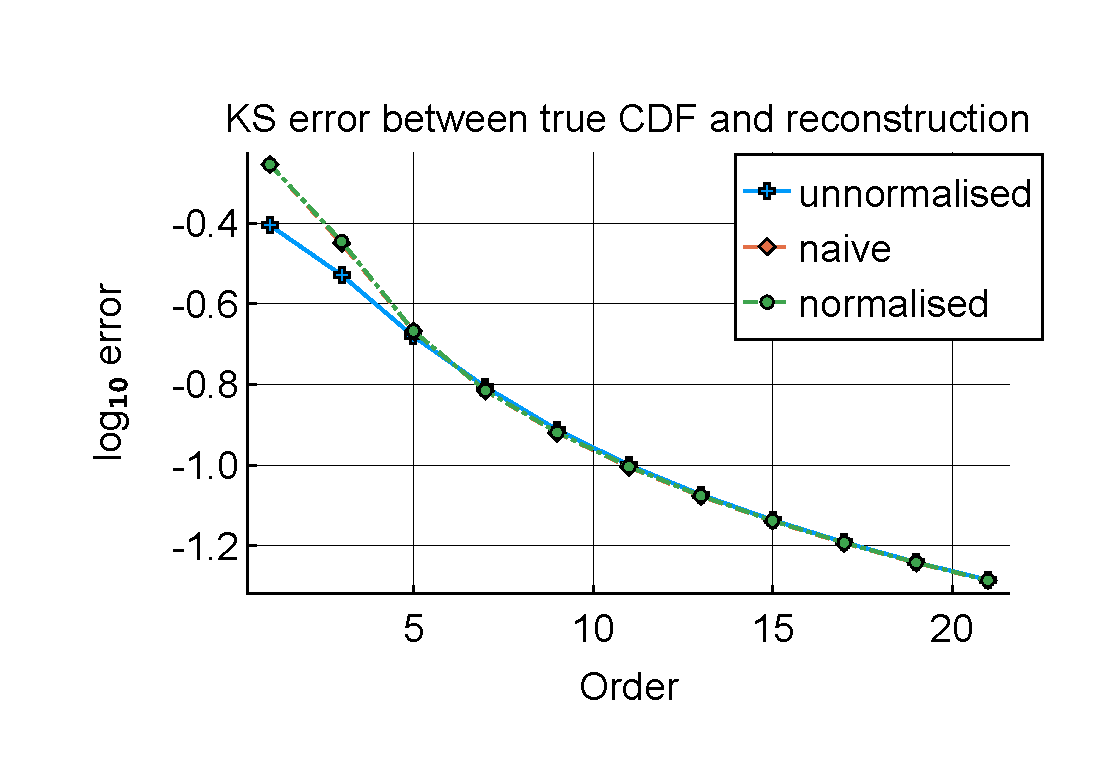
\includegraphics[width=0.5\textwidth,trim={1.25cm 0.8cm 0.25cm 1.25cm},clip]{chapter6/figs/qbdrap_closing_vec/fun2/ks_error_formatted.pdf}%
	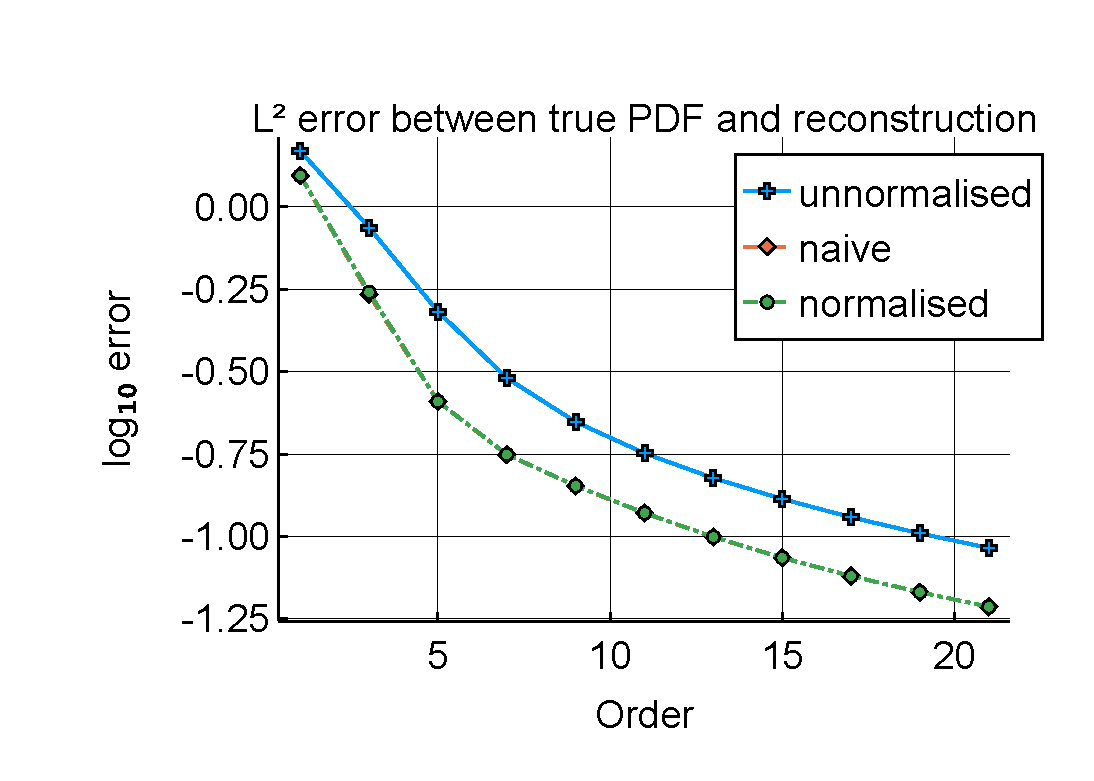
\includegraphics[width=0.5\textwidth,trim={1.25cm 0.8cm 0.25cm 1.25cm},clip]{chapter6/figs/qbdrap_closing_vec/fun2/l2_pdf_error_formatted.pdf}
	\caption{KS error between the true CDF, \(2x1(x<0.5)+1(x\geq 0.5)\), and the approximations (left) and \(L^2\) error between the true PDF, \(2\times 1(x<0.5)\), and the approximations (right) for the three closing vectors considered; unnormalised (blue solid line with crosses), naive normalised (orange dashed line with diamonds) and normalised (green dash-dotted line with circles). The naive normalised (orange) an normalised closing vectors are coincident.}
	\label{fig: fun 2 ks error qbdrap closing vecs}
\end{figure}
\end{example}

\begin{example}Now consider approximating the initial density \(f(x)=1\). Observing Figure~\ref{fig: fun 4 ks error qbdrap closing vecs} of the KS error, and \(L^2\) error between the true initial distribution and the reconstructions, we now see that the normalised reconstructions outperform the unnormalised reconstruction. This suggests that, in this case, the `folding' of closing operator about \(\Delta\) has greatly increased the ability of the reconstruction to approximate this initial distribution. 
\begin{figure}
	\centering
	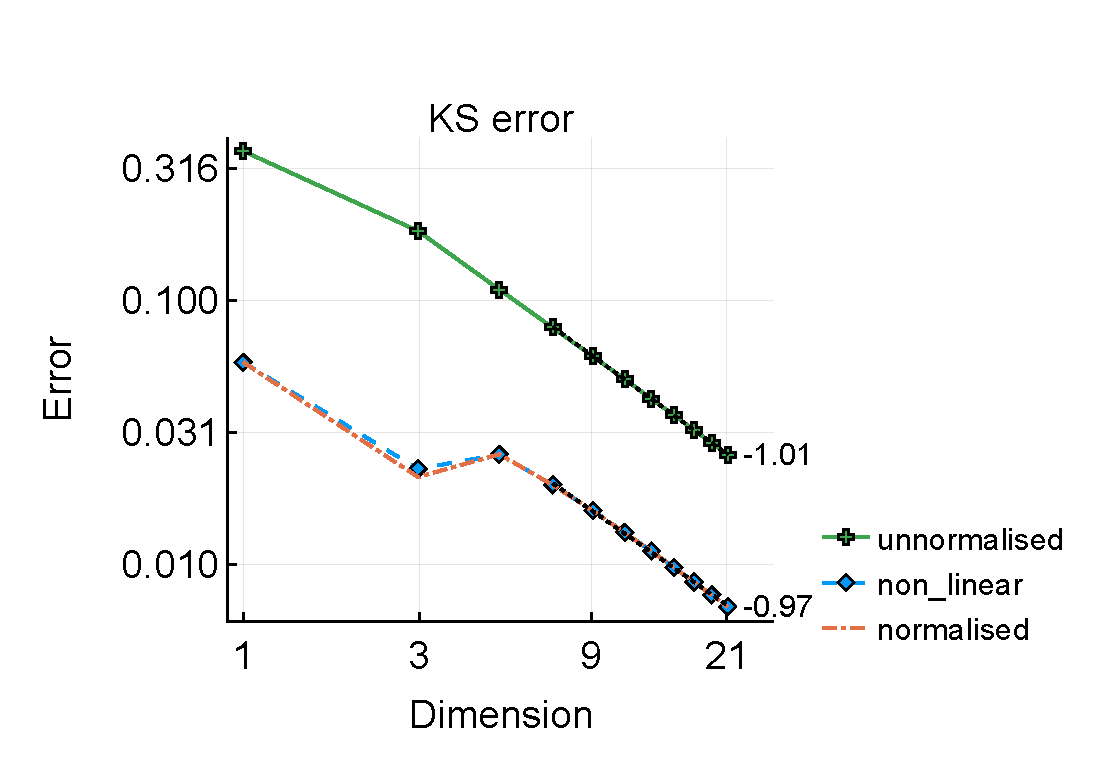
\includegraphics[width=0.5\textwidth,trim={1.25cm 0.8cm 0.25cm 1.25cm},clip]{chapter6/figs/qbdrap_closing_vec/fun4/ks_error_formatted.pdf}%
	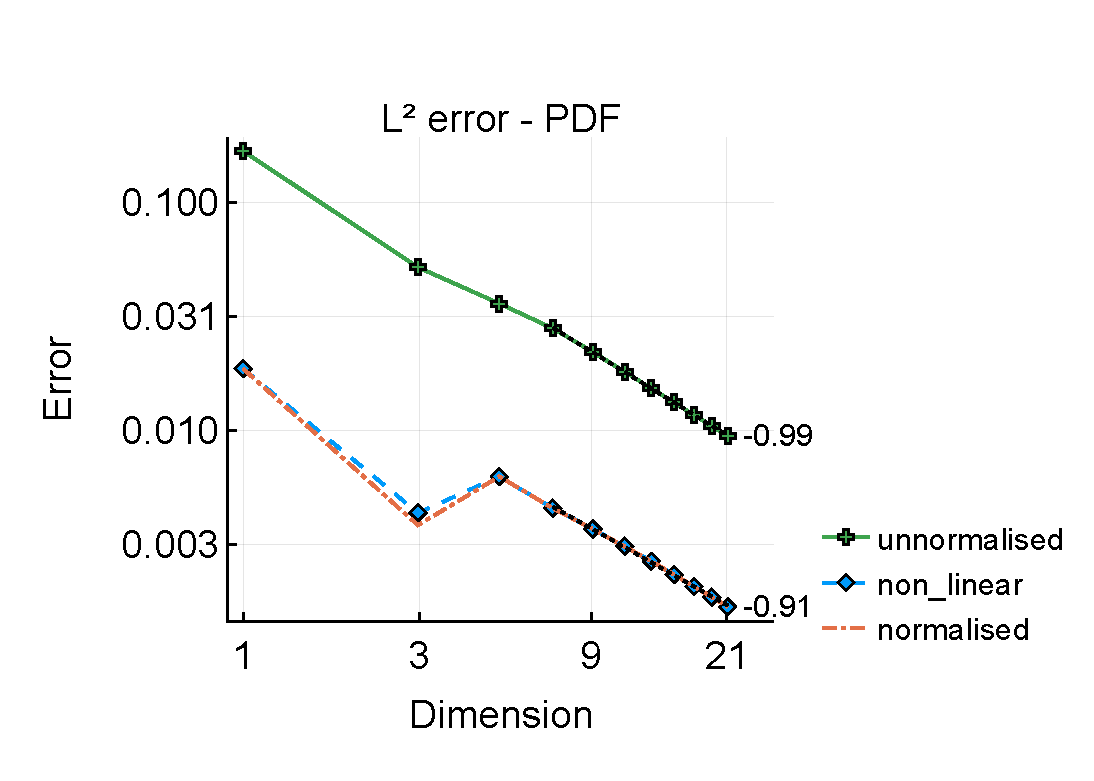
\includegraphics[width=0.5\textwidth,trim={1.25cm 0.8cm 0.25cm 1.25cm},clip]{chapter6/figs/qbdrap_closing_vec/fun4/l2_pdf_error_formatted.pdf}
	\caption{KS error between the true CDF, \(x\), and the approximation (left) and \(L^2\) error between the true PDF and the approximation (right) for the three closing vectors considered; unnormalised (blue solid line with crosses), naive normalised (orange dashed line with diamonds) and normalised (green dash-dotted line with circles). The naive normalised (orange) an normalised closing vectors are coincident.}
	\label{fig: fun 4 ks error qbdrap closing vecs}
\end{figure}

Some insight is gained by looking at Figure~\ref{fig: pdf reconstructed} where we plot the reconstructed PDFs for the unnormalised and normalised closing operators for order 1, 3, 5 and 7, as well as the true PDF. Observing Figure~\ref{fig: pdf reconstructed} notice that the unnormalised reconstruction fails to capture the density at the left of each of the plots and for all orders. This feature is due to a significant amount of mass being lost due to the truncation. In comparison the reconstruction with the normalised closing operator is much better in this region due to the `folding' around \(\Delta\) in the construction of the closing operator. In the reconstruction we also need to allocate the initial condition to a phase with positive rate, or negative rate, so that we can use the appropriate approximation and reconstruction method as discussed in Section~\ref{sec: closing}. Here we suppose that the phase is positive, so the `folding' around \(\Delta\) in the normalised closing operators appears appears at the left of the plots. In general, reconstructions via the unnormalised closing operator typically underestimate the value of the function in this region. 

Figure~\ref{fig: pdf reconstructed} also show that both closing operators do not approximate the initial condition well at the right-hand side of the interval. This is a common feature, and drawback, of the QBD-RAP method. Perhaps there is a different reconstruction method or yet another closing operator which could alleviate this issue. 
\begin{figure}
	\centering
	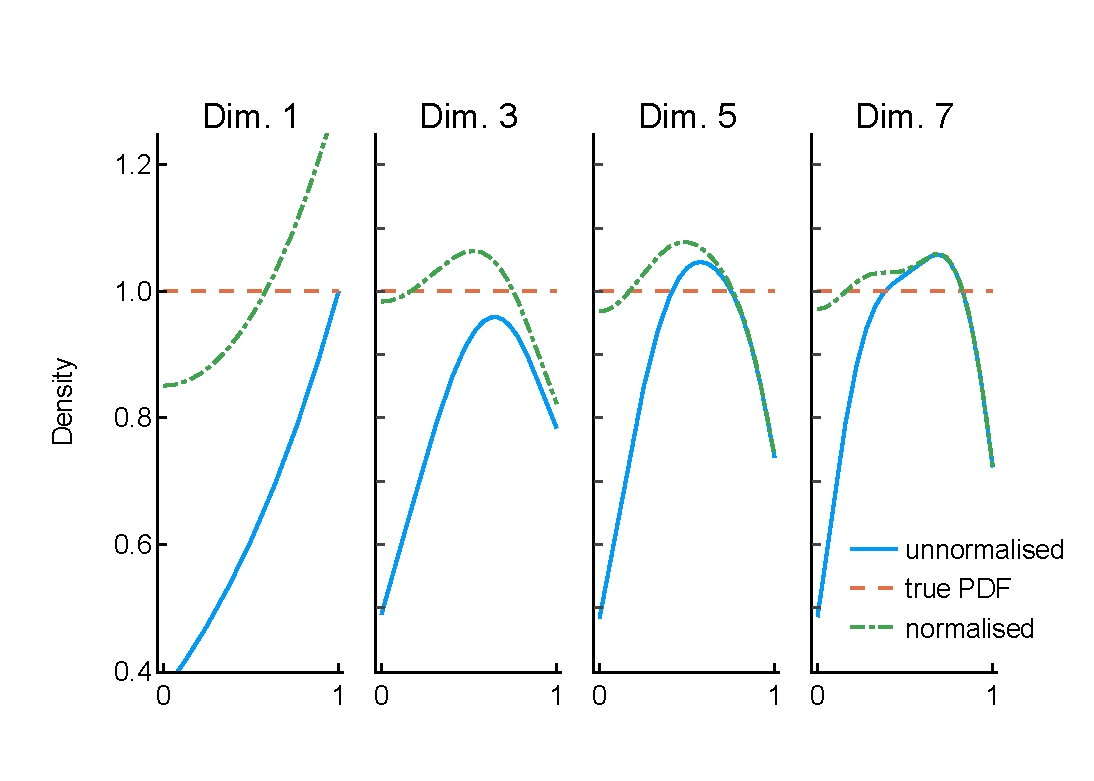
\includegraphics[width=\textwidth]{chapter6/figs/qbdrap_closing_vec/fun4/pdfs_formatted.pdf}
	\caption{Reconstructed PDFs using the unnormalised closing operator (blue solid line), normalised closing operator (green dash-dotted line), for various orders, and the true PDF which is \(f(x)=1\) (orange dashed line).}
	\label{fig: pdf reconstructed}
\end{figure} 
\end{example}

\begin{example}Next we consider approximating the initial distribution with density \(-6x^2+6x\). Observing the left-hand panel of Figure~\ref{fig: fun 6 ks error qbdrap closing vecs}, which plots the KS error against the order of the reconstruction for the three closing operators, we once again see that the reconstruction using the unnormalised closing operator performs the worst, while the performance of the two normalised reconstructions is indistinguishable. However, if we instead look at the right-hand panel of Figure~\ref{fig: fun 6 ks error qbdrap closing vecs}, which plots the \(L^2\) error between the reconstructed PDF and the true PDF, we see that with this metric, then unnormalised closing operator performs better than the two normalised ones for orders 5 and above. 
\begin{figure}
	\centering
	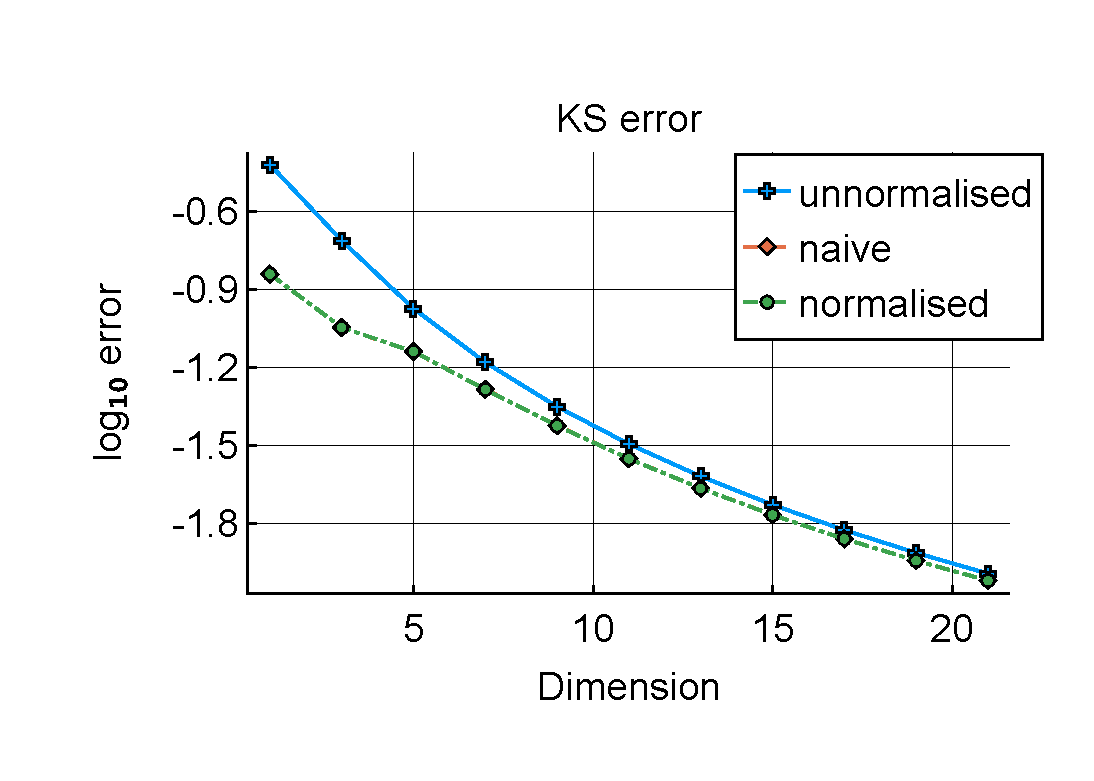
\includegraphics[width=0.5\textwidth,trim={1.25cm 0.8cm 0.25cm 1.25cm},clip]{chapter6/figs/qbdrap_closing_vec/fun6/ks_error_formatted.pdf}%
	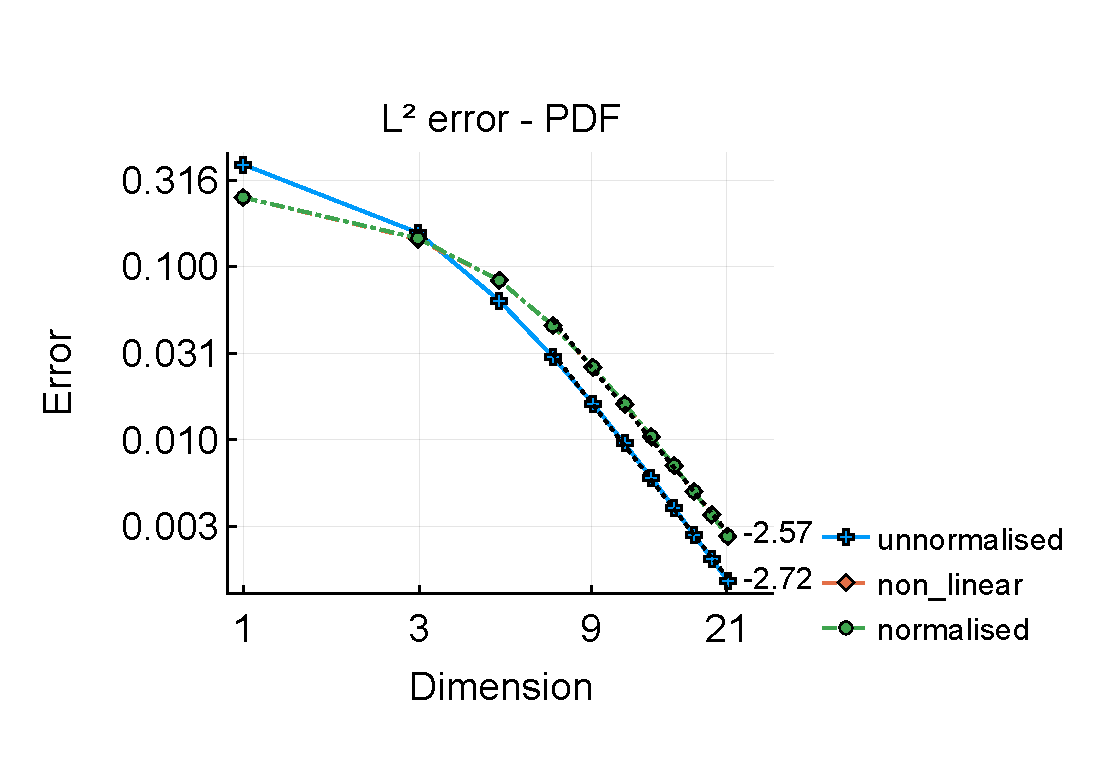
\includegraphics[width=0.5\textwidth,trim={1.25cm 0.8cm 0.25cm 1.25cm},clip]{chapter6/figs/qbdrap_closing_vec/fun6/l2_pdf_error_formatted.pdf}
	\caption{KS error between the true CDF, \(-2x^3+3x^2\), and the approximation (left) and \(L^2\) error between the true PDF \(-6x^2+6x\) and the approximation (right), for the three closing vectors considered; unnormalised (blue solid line with crosses), naive normalised (orange dashed line with diamonds) and normalised (green dash-dotted line with circles). The naive normalised (orange) an normalised closing vectors are coincident.}
	\label{fig: fun 6 ks error qbdrap closing vecs}
\end{figure}

The fact that the unnormalised closing operator outperforms the two normalised ones can be explain, once again, by the fact that, for the normalised operators we have `folded' the ME density function back on itself. In Figure~\ref{fig: pdf reconstructed quadratic} we plot the unnormalised and normalised reconstructions along with the true PDF, \(-6x^2+6x\). In Figure~\ref{fig: pdf reconstructed quadratic} we observe that, at the left of the plot, the normalised reconstructions over estimate the density function in this region, where as the unnormalised reconstruction looks to be doing better. Recall that the `folding' in the normalised closing operator manifest itself as extra mass at the left of these plots compared to the unnormalised reconstructions. 
\begin{figure}
	\centering
	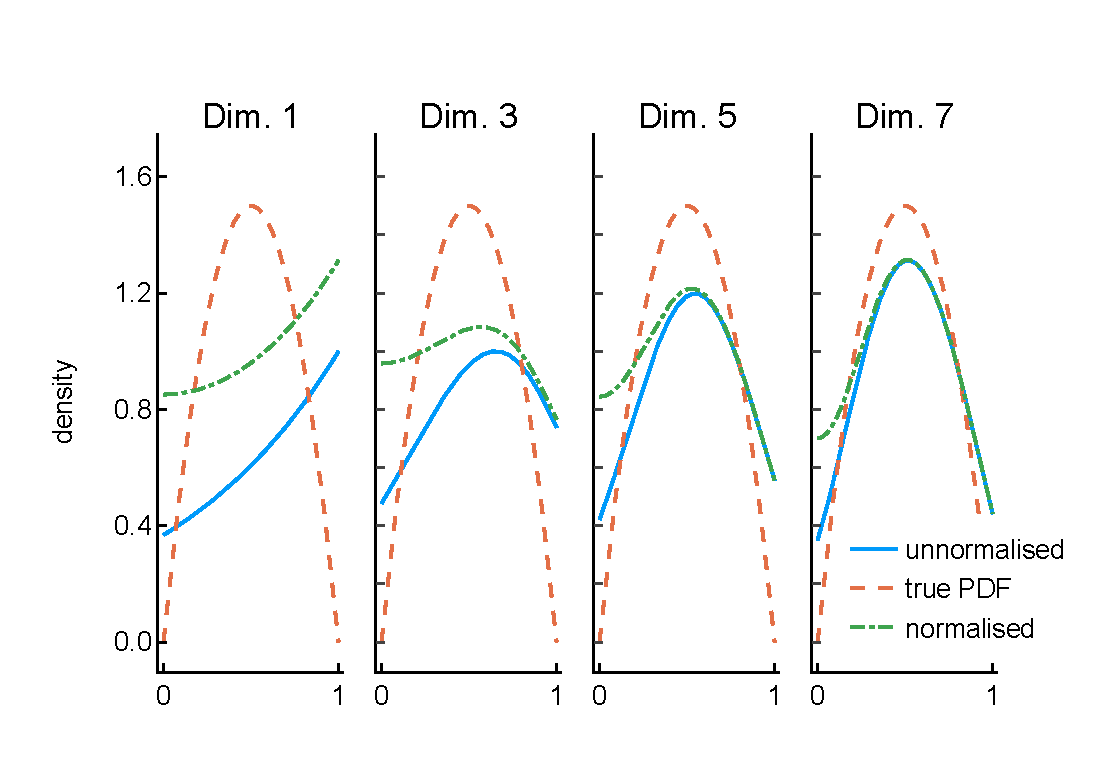
\includegraphics[width=\textwidth]{chapter6/figs/qbdrap_closing_vec/fun6/pdfs_formatted.pdf}
	\caption{Reconstructed PDFs using the unnormalised closing operator (blue solid line), normalised closing operator (green dash-dotted line), for various orders, and the true PDF which is \(f(x)=-6x^2+6x\) (orange dashed line).}
	\label{fig: pdf reconstructed quadratic}
\end{figure} 
\end{example}

\begin{example}Lastly, we consider approximating the initial distribution with PDF \(3e^{-3x}/(1-e^{-3})\). This density function is at a maximum at the left of the region. Considering what we have learnt so far about the unnormalised operator underestimating in this region, we expect that the unnormalised closing operator will perform relatively poorly in this case. Indeed, observing Figures~\ref{fig: fun 7 ks error qbdrap closing vecs} we see that the normalised reconstructions perform relatively well compared to the unnormalised reconstruction as measured by both error metrics (KS statistic and \(L^2\) norm on the PDF). If we observed plots of the PDFs (omitted), we would once again see that this is due to the loss of mass at the left-hand side of the region due to the truncation. 
\begin{figure}
	\centering
	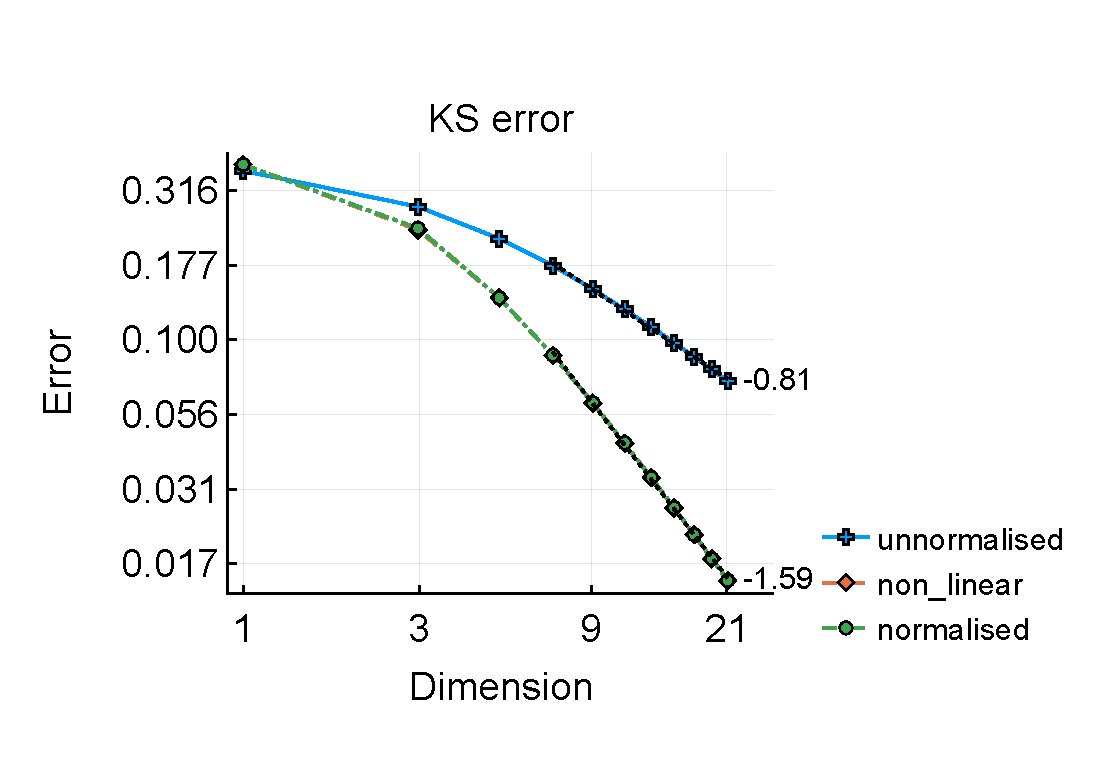
\includegraphics[width=0.5\textwidth,trim={1.25cm 0.8cm 0.25cm 1.25cm},clip]{chapter6/figs/qbdrap_closing_vec/fun7/ks_error_formatted.pdf}%
	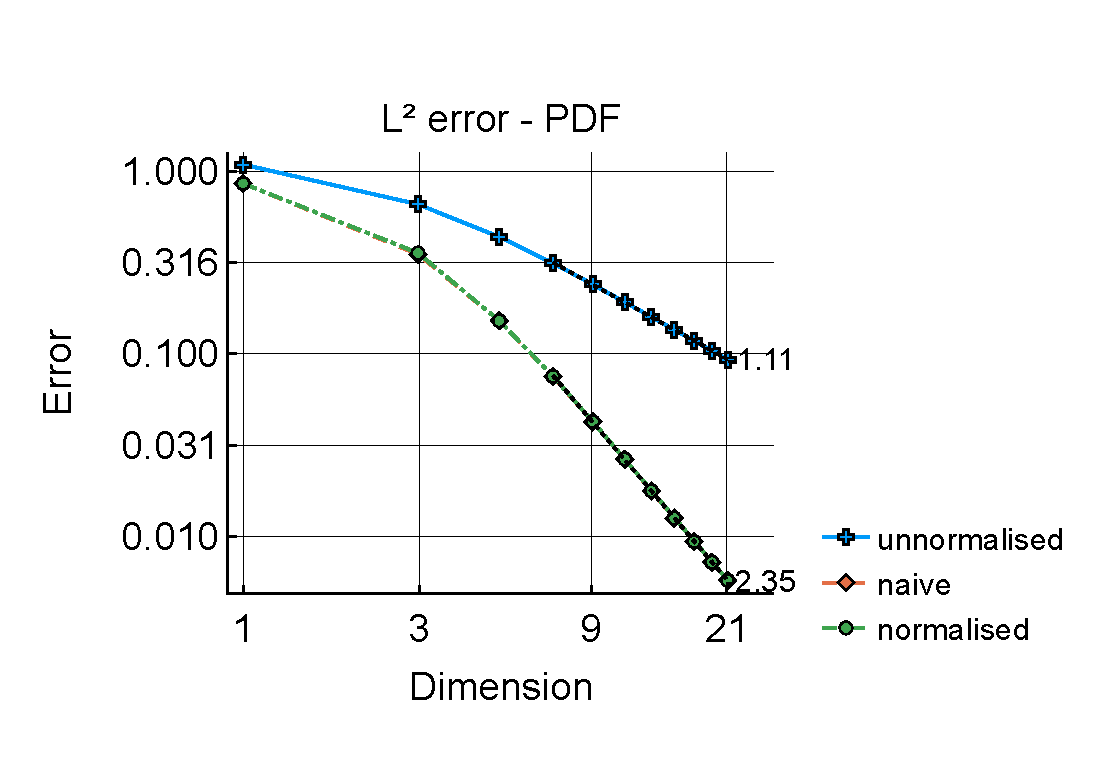
\includegraphics[width=0.5\textwidth,trim={1.25cm 0.8cm 0.25cm 1.25cm},clip]{chapter6/figs/qbdrap_closing_vec/fun7/l2_pdf_error_formatted.pdf}
	\caption{KS error between the true CDF, \((1-e^{-3x})/(1-e^{-3})\), and the approximation (left) and \(L^2\) error between the true PDF and the approximation for the three closing vectors considered; unnormalised (blue solid line with crosses), naive normalised (orange dashed line with diamonds) and normalised (green dash-dotted line with circles). The naive normalised (orange) an normalised closing vectors are coincident.}
	\label{fig: fun 7 ks error qbdrap closing vecs}
\end{figure}
\end{example}

Given the evidence above we choose to use the normalised closing operator to reconstruct solutions. Further, unlike the naive normalised operator, the normalised operator is theoretically justified in that we proved the closing operator leads to a convergent scheme and is linear. 

\subsection{Comparison of methods}\label{sec: comp}
Here we compare the ability of the QBD-RAP, uniformisation, and DG methods to reconstruct initial conditions. 

\begin{example}First we consider the initial condition with CDF \(1(x\geq 0.5)\), that is, a point mass at 0.5. This distribution does not have a PDF so we can compare the CDFs only. In Figure~\ref{fig: fun 1 comp} we plot the KS metric (left) and \(L^1\) metric (right) between the true CDF and the reconstructed approximations. Observing the KS metric, it appears that none of the methods converge and the KS error sits around 0.5. This reflects the fact that convergence in distribution implies point-wise convergence of the CDFs except at points of discontinuity. None of the methods appear to converge at this point. Observing the \(L^1\) error between the true CDF and reconstructed approximation (which is the area between the two CDFs) we now see that the methods appear to show the convergent behaviour we expect. Here, the uniformisation method appears to perform the best, while the QBD-RAP method performs the worst. The rate of convergence of the QBD-RAP method appears to be similar to the rate of convergence of the DG scheme. 

Perhaps it is no surprise that the uniformisation method performs best. In the uniformisation method as we increase the order, we partition the cell \([0,1]\) into smaller sub-cells, and use constant functions on each sub-cell to approximate the function. As such, the uniformisation method can produce a piecewise continuous, linear approximation to the CDF. In contrast, both the DG and QBD-RAP methods result in a smooth approximation to the CDF. 
\begin{figure}
	\centering
	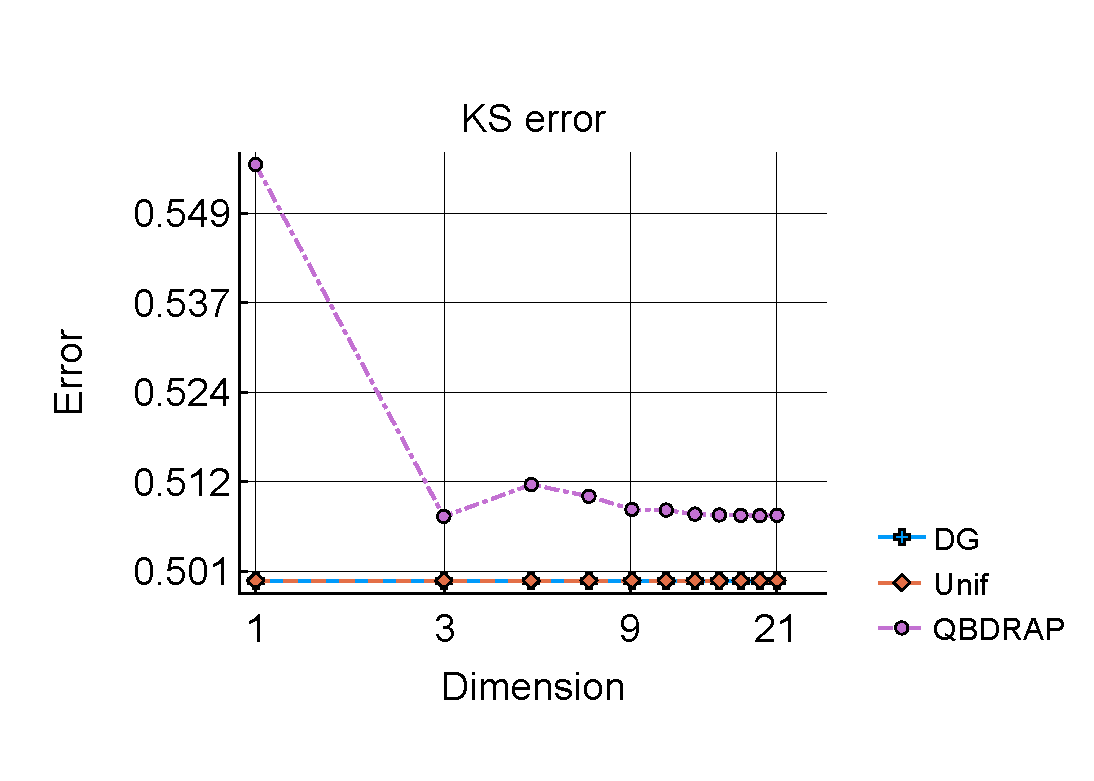
\includegraphics[width=0.5\textwidth,trim={1.25cm 0.8cm 0.25cm 1.25cm},clip]{chapter6/figs/comp/fun1/meshs_ks_error_formatted.pdf}%
	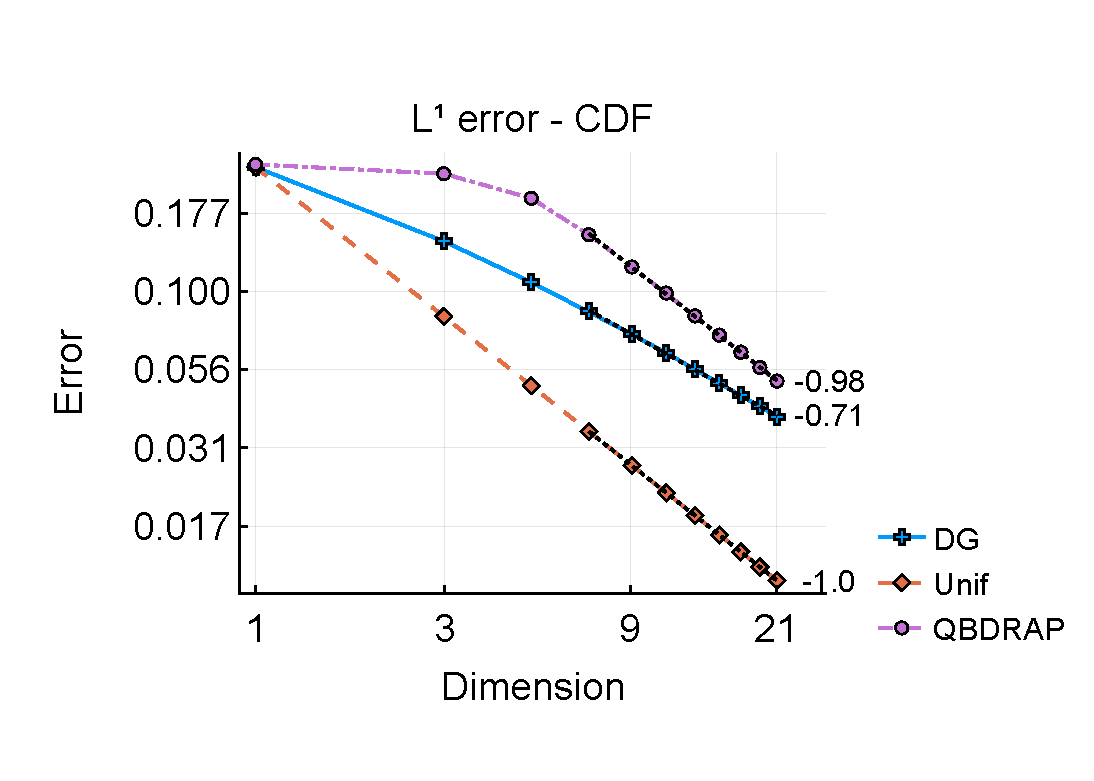
\includegraphics[width=0.5\textwidth,trim={1.25cm 0.8cm 0.25cm 1.25cm},clip]{chapter6/figs/comp/fun1/meshs_l1_cdf_error_formatted.pdf}
	\caption{KS error between the true CDF, \(1(x\geq 0.5)\), and the approximations (left) and \(L^1\) error between the true CDF and the approximations for the DG method (blue solid line with crosses), uniformisation method (orange dashed line with diamonds) and QBD-RAP method (green dash-dotted line with circles).}
	\label{fig: fun 1 comp} 
\end{figure}

In Figure~\ref{fig: pdf comp fun 1} we plot the approximated CDFs for the DG, uniformisation and QBD-RAP methods alongside the true CDF. The DG method displays undesirable features for an approximation to a CDF -- it is not monotonically increasing, at some points it is negative and at some points it is above 1. On the other hand, although the QBD-RAP method converges slowest, it displays good properties in that it results in a monotonically increasing CDF, starting at 0 and ending at 1. 
\begin{figure}
	\centering
	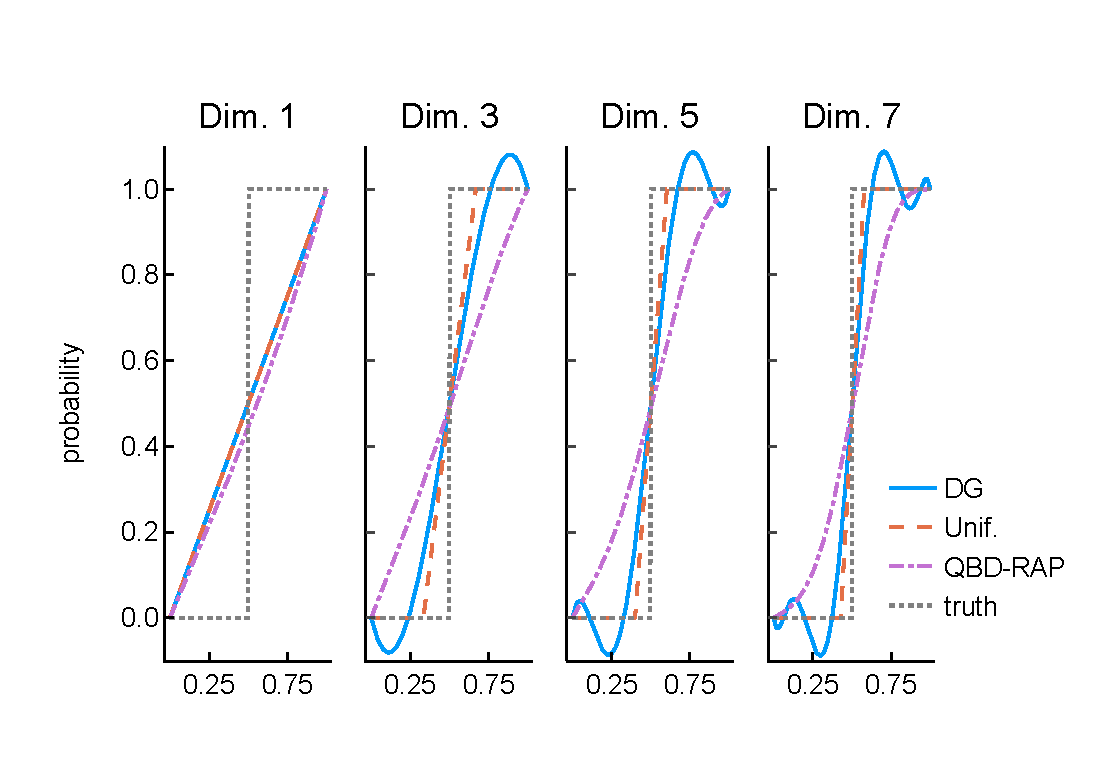
\includegraphics[width=\textwidth]{chapter6/figs/comp/fun1/cdfs_formatted.pdf}
	\caption{Reconstructed CDFs using the DG (blue solid line), uniformisation (orange dashed line) and QBD-RAP (green dot-dashed line) methods. The true distribution function is \(1(x\geq 0.5)\) (grey dotted line).}
	\label{fig: pdf comp fun 1}
\end{figure} 
\end{example}

\begin{example}Now consider approximating the initial distribution with PDF \(1(x\leq 0.5)\). Figure~\ref{fig: fun 2 comp} plots the KS error (left) and \(L^2\) error between the true and approximate PDFs (right). Figure~\ref{fig: fun 2 comp} suggests that all methods converge at a similar rate for this problem. Once again, the QBD-RAP method performs worst, the uniformisation method second, and the DG method the best. However, once again the DG method exhibits undesirable properties -- the approximation to the CDF is, at some points above 1, is not monotonic, though these violations are not as severe in this case as they were for the case above. 
\begin{figure}
	\centering
	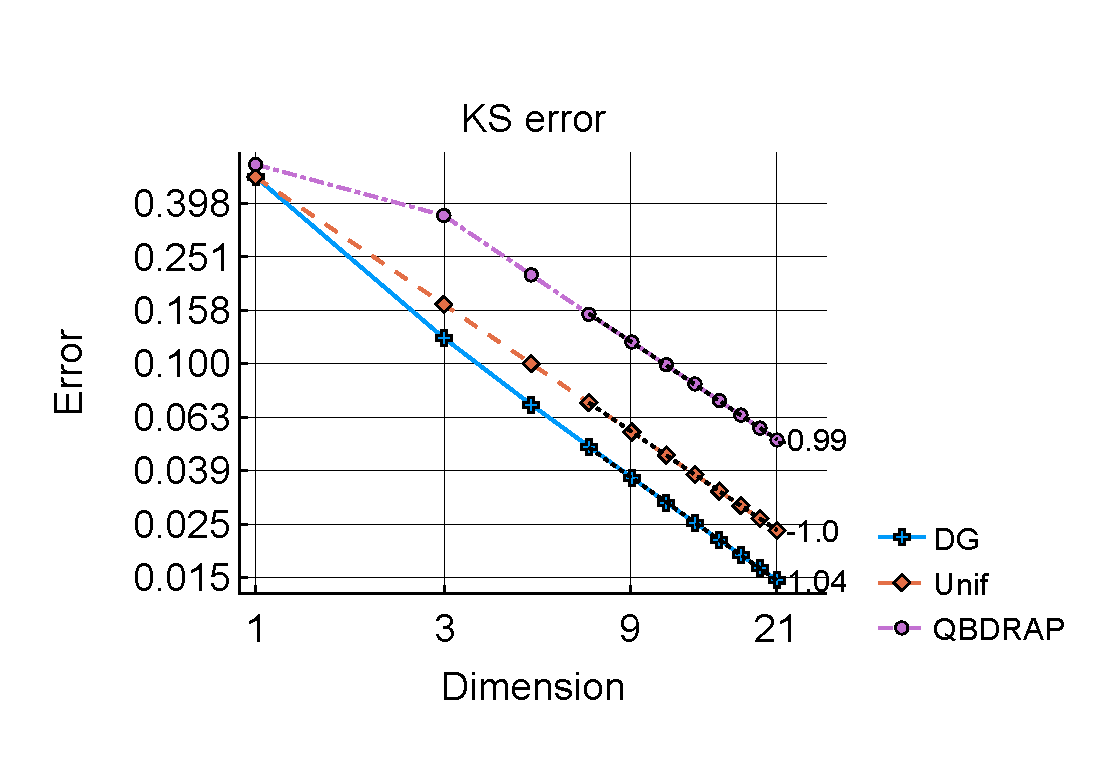
\includegraphics[width=0.5\textwidth,trim={1.25cm 0.8cm 0.25cm 1.25cm},clip]{chapter6/figs/comp/fun2/meshs_ks_error_formatted.pdf}%
	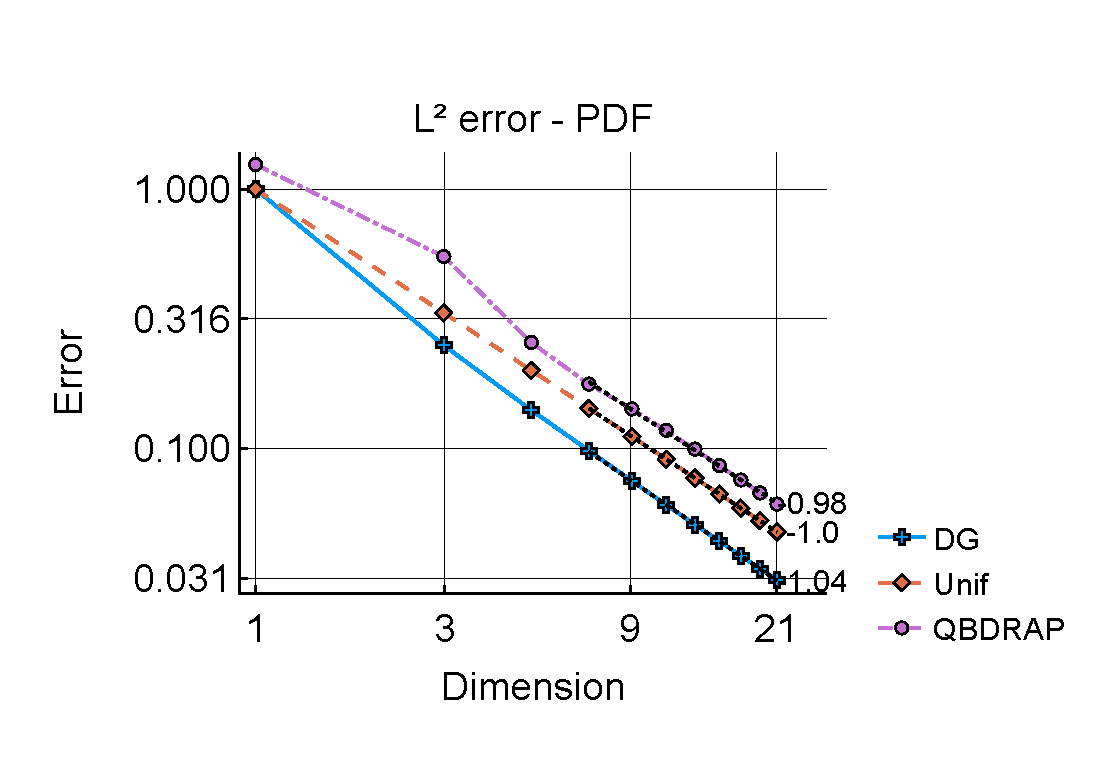
\includegraphics[width=0.5\textwidth,trim={1.25cm 0.8cm 0.25cm 1.25cm},clip]{chapter6/figs/comp/fun2/meshs_l2_pdf_error_formatted.pdf}
	\caption{KS error between the true CDF and the approximations (left) and \(L^2\) error between the true PDF, \(1(x\geq 0.5)\), and the approximations for the DG method (blue solid line with crosses), uniformisation method (orange dashed line with diamonds) and QBD-RAP method (green dash-dotted line with circles).}
	\label{fig: fun 2 comp} 
\end{figure}
\end{example}

\begin{example}So far we have considered two problems which exhibit discontinuities. At the other extreme we now consider an initial distribution with density \(-6z^2+6x\). In Figure~\ref{fig: fun 6 comp} we plot the KS error and the \(L^2\) error between the true and approximated PDF. Since the DG method projects the initial condition onto a polynomial basis, then, for an order 3 approximation and above, the DG method can theoretically approximate the initial condition exactly. This is reflected in Figure~\ref{fig: fun 6 comp}, where the blue curve drops sharply from 1-3, then plateaus. Due to numerical integration errors, for example in the evaluation of the integral in the \(L^2\) norm, and due to machine arithmetic, the errors for the DG scheme are not 0. Regarding the other two methods, they too appear to be convergent at approximately the same rate, with the uniformisation method perform better for the KS error, but very similarly in terms of the \(L^2\) error. 
\begin{figure}
	\centering
	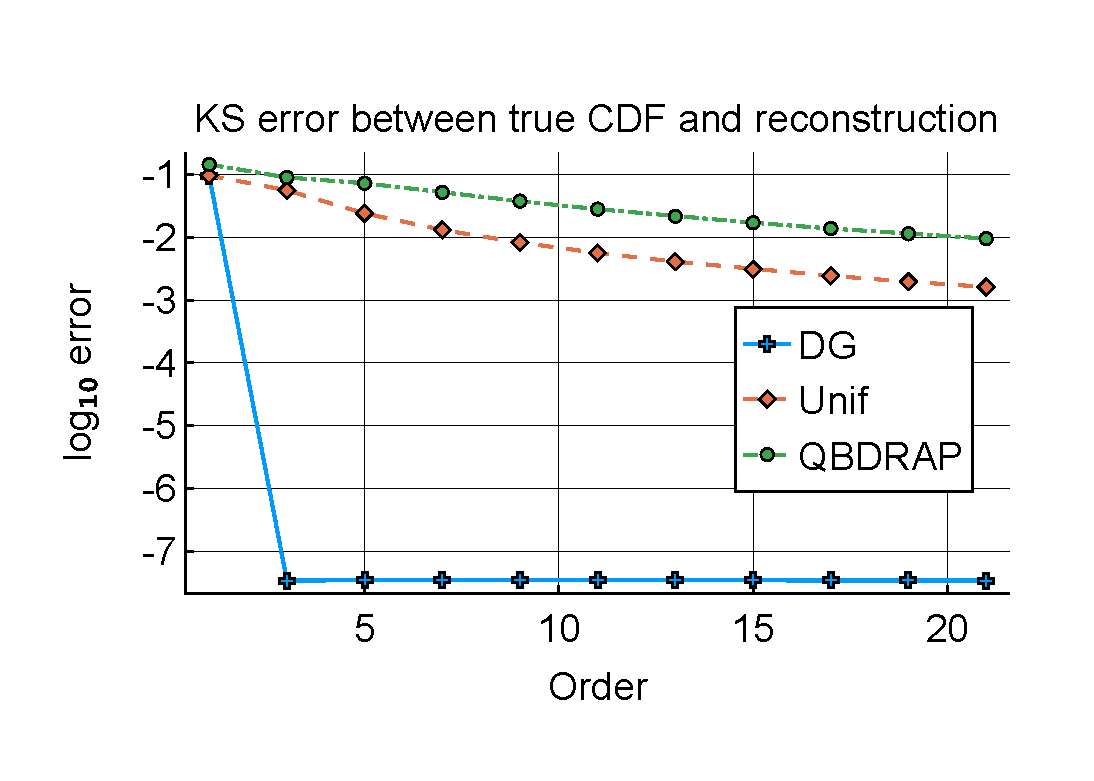
\includegraphics[width=0.5\textwidth,trim={1.25cm 0.8cm 0.25cm 1.25cm},clip]{chapter6/figs/comp/fun6/meshs_ks_error_formatted.pdf}%
	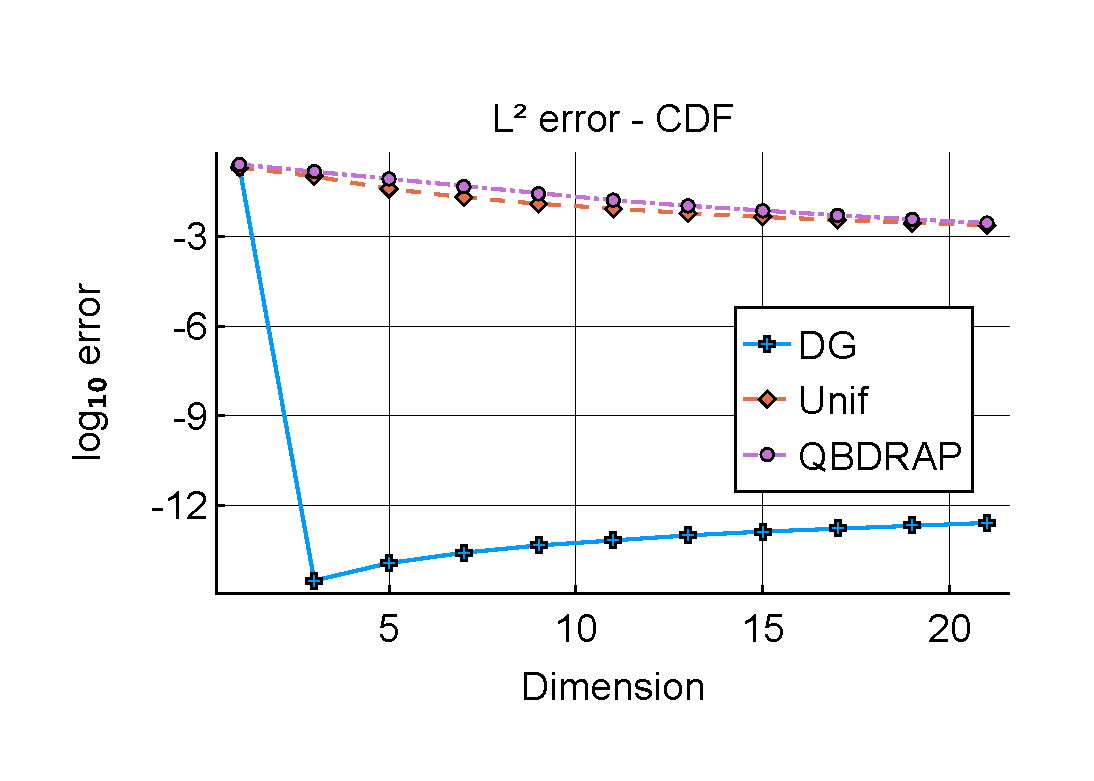
\includegraphics[width=0.5\textwidth,trim={1.25cm 0.8cm 0.25cm 1.25cm},clip]{chapter6/figs/comp/fun6/meshs_l2_pdf_error_formatted.pdf}
	\caption{KS error between the true CDF and the approximations (left) and \(L^2\) error between the true PDF, \(-6z^2+6x\), and the approximations for the DG method (blue solid line with crosses), uniformisation method (orange dashed line with diamonds) and QBD-RAP method (green dash-dotted line with circles).}
	\label{fig: fun 6 comp} 
\end{figure}
\end{example}

\begin{example}Consider now the initial distribution with PDF \(cos(4\pi(x+0.5))+1\). Figure~\ref{fig: fun 9 comp} shows the errors. Both the KS error (left) and \(L^2\) norm between the true and approximated PDFs tell a similar story. For sufficiently high order, the DG method approximates the inital condition very well. The uniformisation method performs second best, while the QBD-RAP method is slowest to converge. 
\begin{figure}
	\centering
	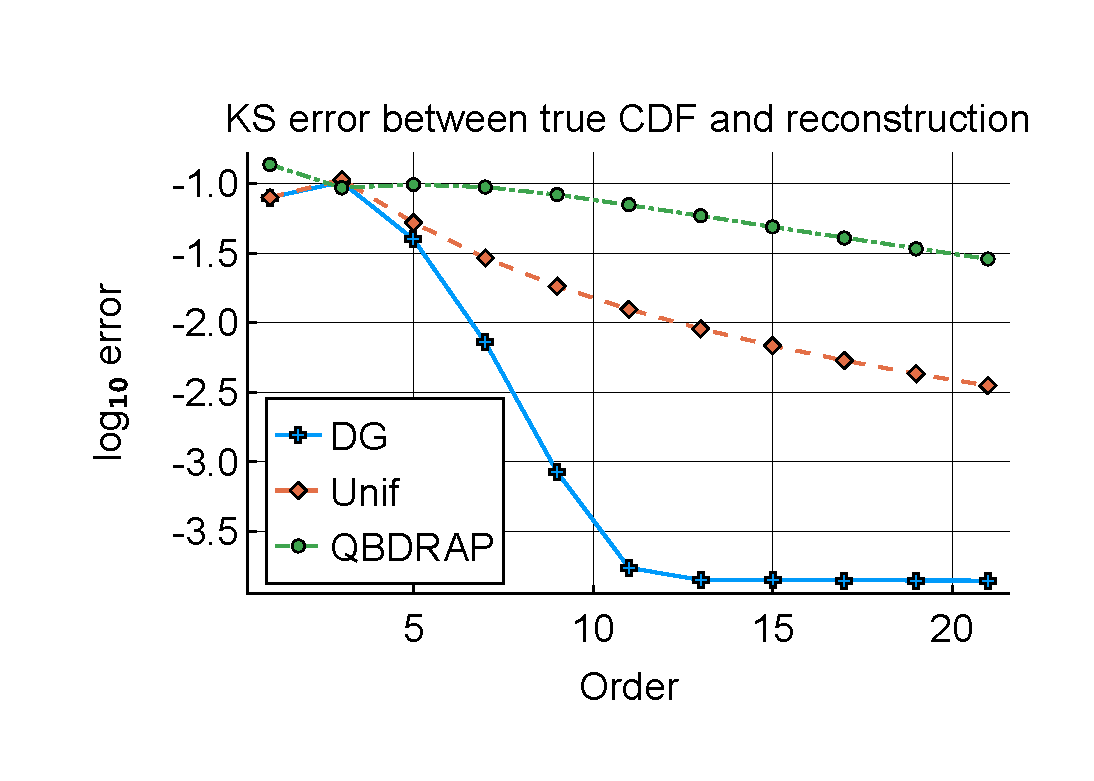
\includegraphics[width=0.5\textwidth,trim={1.25cm 0.8cm 0.25cm 1.25cm},clip]{chapter6/figs/comp/fun9/meshs_ks_error_formatted.pdf}%
	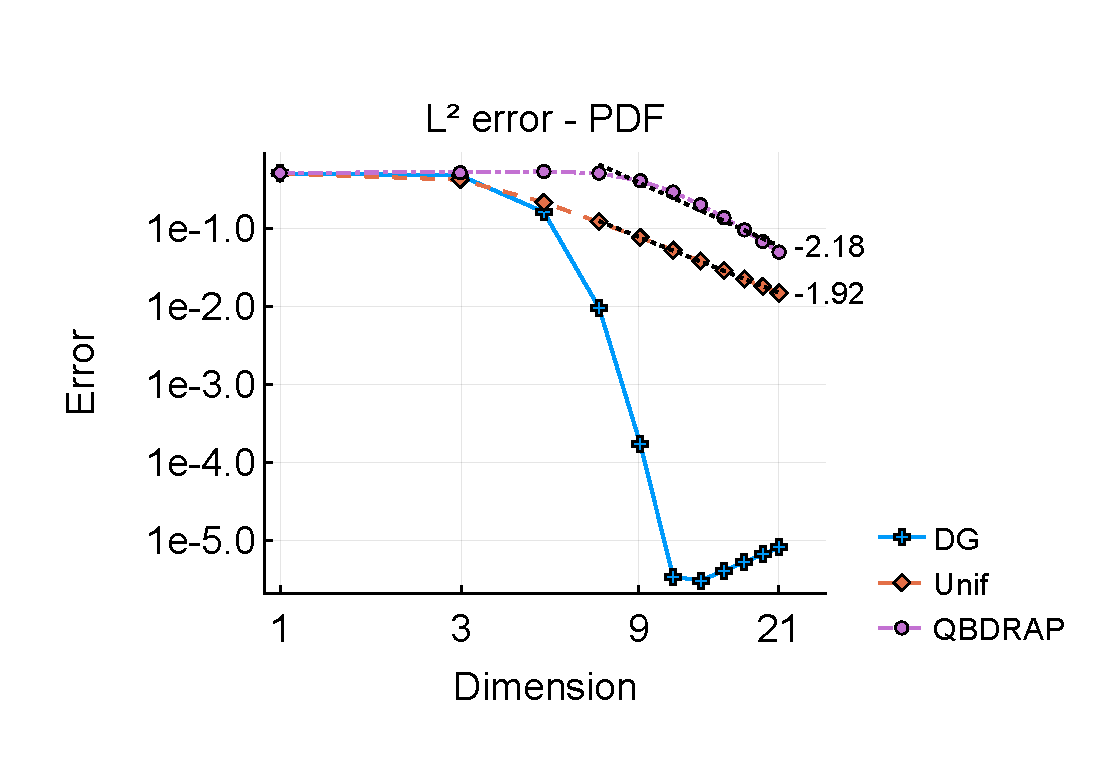
\includegraphics[width=0.5\textwidth,trim={1.25cm 0.8cm 0.25cm 1.25cm},clip]{chapter6/figs/comp/fun9/meshs_l2_pdf_error_formatted.pdf}
	\caption{KS error between the true CDF and the approximations (left) and \(L^2\) error between the true PDF, \(cos(4\pi(x+0.5))+1\), and the approximations for the DG method (blue solid line with crosses), uniformisation method (orange dashed line with diamonds) and QBD-RAP method (green dash-dotted line with circles).}
	\label{fig: fun 9 comp} 
\end{figure}
\end{example}
\FloatBarrier

\section{Travelling wave}
Here we investigate the performance the different schemes for approximating transient distributions of one-dimensional travelling wave problems with varying initial conditions. Consider a (trivial) fluid queue with one phase, generator \(\bs T=[0]\) and rate \(c=1\). The PDE (if/when it exists) which describes this system is 
\[\cfrac{\partial}{\partial t} f(x,t) = -\cfrac{\partial}{\partial x} f(x,t),\]
where \(f(x,t)\) is the density at time \(t\). Given an initial condition, \(f(x,0)\), solutions to this problem are given by 
\[f(x,t) = f(x-t,0)\]
so the solution at time \(t\) is just a shift in the initial condition \(t\) units to the right. We suppose that the fluid queue is bounded, with a lower boundary \(x=0\) and upper boundary \(x=10\). 

We use the QBD-RAP, uniformisation and DG schemes to discretise the solution in space. We discretise the interval \([0,10]\) into \(10\) cell, each of width 1. We use \(10,001\) points to approximate the integrals which appear in the construction of the initial conditions, to approximate the integrals appearing in the error metrics, and also as a set of discrete points on which evaluate the CDFs to approximate the KS metric. We use the SSPRK4 method to integrate over time using a step size of \(0.005\), and we evolve the system until time \(t=4\). For the DG method we also implement the Generalise MUSCL (REF, appendix?) slope limiter to stabilise the integration. 

\begin{example}First consider the initial condition with PDF \(1(x<1)\). The level of the fluid queue is uniformly distributed over the first cell. For the DG and uniformisation methods, the initial condition can be represented exactly, whereas, for the QBD-RAP method, it cannot. Thus, in this case, there is no discretisation error in constructing the initial condition for the DG and uniformisation methods. Furthermore, at time \(t=4\), the solution in \(1(x\in[4,5)\), and the projections related to the DG and uniformisation methods can represent this solution exactly too.

Figure~\ref{fig: fun 4 wave} plots the KS error between the approximated and true CDFs and \(L^2\) error between the approximated and true PDFs. The DG method with the MUSCL limiter does not appear to converge for this problem. This is caused by the limiter reducing the method to linear in when oscilations are deteced, so increasing the order does not increase the accuracy of the method. The other two positivity preserving methods, the uniformisation method and QBD-RAP methods, both appear to be converging, with the QBD-RAP method converging faster. With these error metrics, the DG method also appears to converge. However, if we observe the solutions resulting from the DG method (Figure~\ref{fig: pdf wave fun 4} top-row), we find them to be unsatisfactory due to oscilations and negative values. 

Figure~\ref{fig: pdf wave fun 4} plots the density functions reconstructed using the DG, uniformisation, DG with MUSCL limiter and QBD-RAP methods. In the first row we observe that the DG method (sans limiter) produces an approximation to the PDF with negative values for orders greater than 1. In the third row of Figure~\ref{fig: pdf wave fun 4} we observe that, with the limiter the approximation does not change significantly after order 3. This is due the the fact that the DG method is at best linear. In the second row of Figure~\ref{fig: pdf wave fun 4} is the solution approximated using the uniformisation method, and in the last row is the solution approximated using the QBD-RAP method. 
\begin{figure}
	\centering
	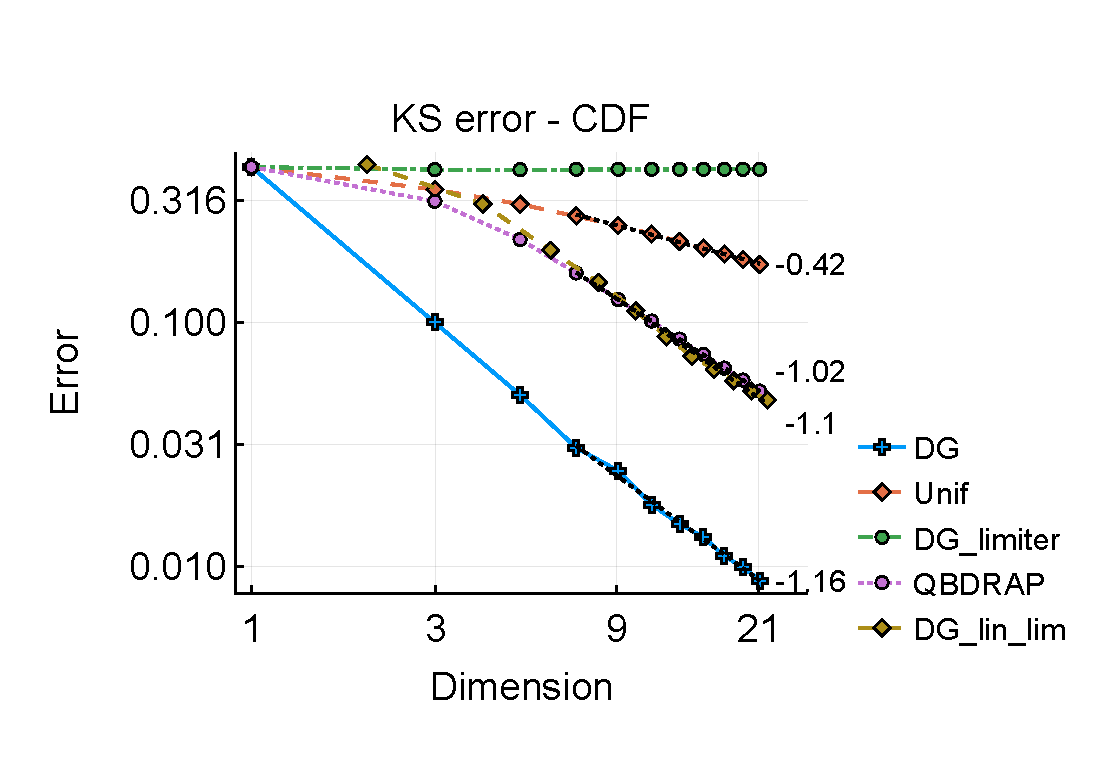
\includegraphics[width=0.5\textwidth,trim={0.75cm 0.8cm 0.25cm 1.25cm},clip]{chapter6/figs/wave/fun4/meshs_ks_error_formatted.pdf}%
	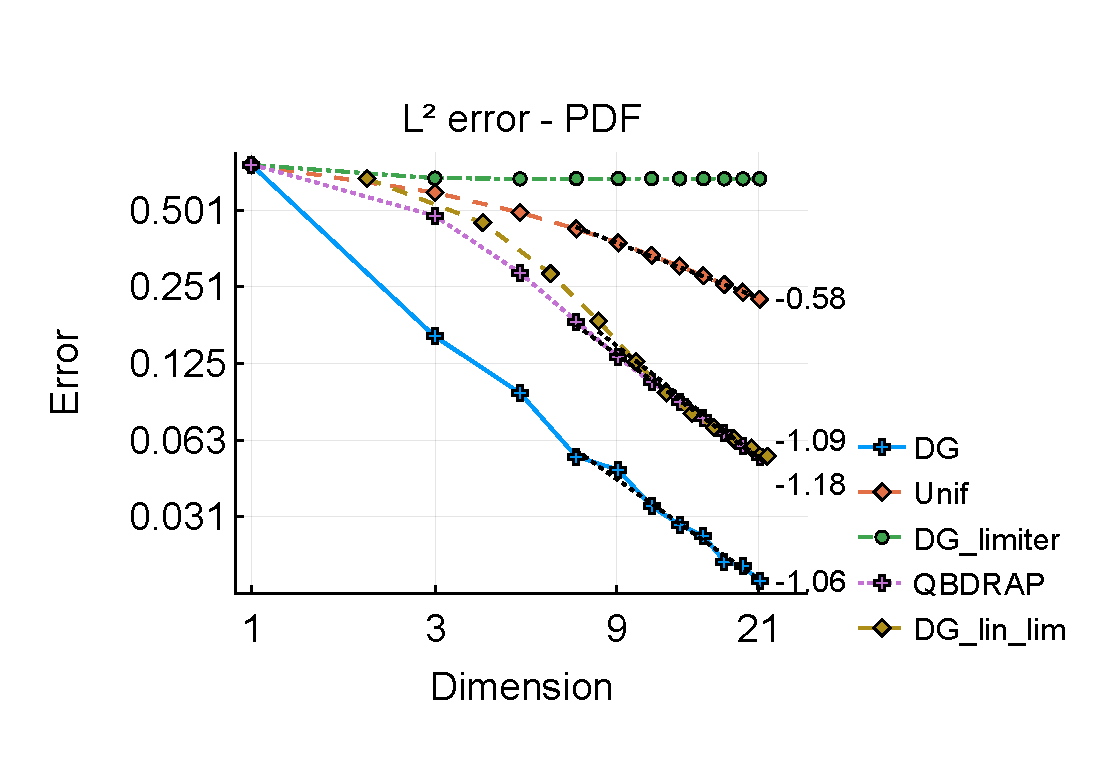
\includegraphics[width=0.5\textwidth,trim={0.75cm 0.8cm 0.25cm 1.25cm},clip]{chapter6/figs/wave/fun4/meshs_l2_pdf_error_formatted.pdf}
	\caption{KS error between the true CDF and the approximations (left) and \(L^2\) error between the true PDF, \(1(4\leq x < 5)\), and the approximations for the DG method (blue solid line with crosses), DG method with the MUSCL limiter (green dash-dotted line with crosses), uniformisation method (orange dashed line with diamonds) and QBD-RAP method (green dash-dotted line with circles).} 
	\label{fig: fun 4 wave} 
\end{figure}
\begin{figure}
	\centering
	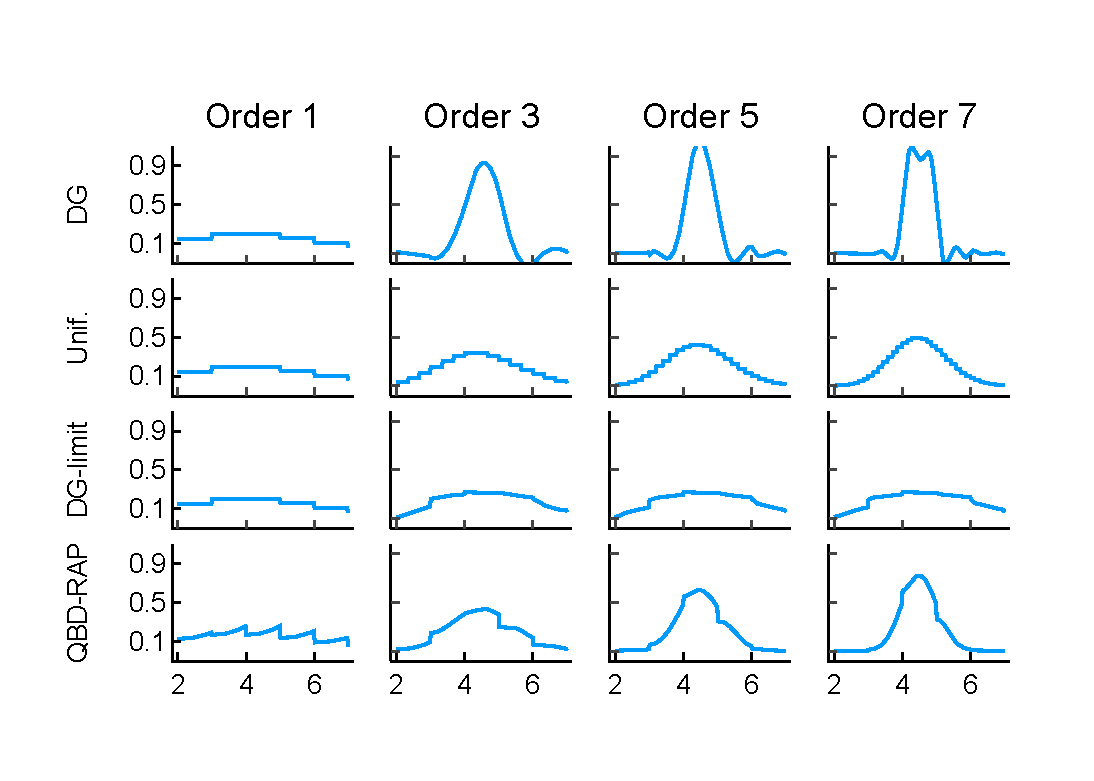
\includegraphics[width=\textwidth]{chapter6/figs/wave/fun4/pdfs_formatted.pdf}
	\caption{Reconstructed PDFs using the DG (top row), uniformisation (second row), DG with MUSCL limiter (third row) and QBD-RAP (bottom row) methods, for order 1, 3, 5, and 7 (columns). The true density function is \(1(4\leq x<5)\).}
	\label{fig: pdf wave fun 4}
\end{figure} 

This is a particularly interesting example. It shows that, for the DG method, even though there is no discretisation error for the initial condition, we have use a strong stability preserving time-intergration method, and the projection off which the DG method is based can represent the transient distribution at time \(t=4\) exactly, there is still the possibility of badly behaved solutions as in the top row of Figure~\ref{fig: pdf wave fun 4}. 
\end{example}

\begin{example}Another interesting example occurs with the initial condition with CDF \(1(z\geq 0.5)\), i.e.~a point mass at 0.5. The exact solution at time \(t=4\) is therefore a point mass at \(4.5\). No PDF exists for the true distribution, so instead we compare the CDFs. Moreover, when we analysed reconstruction of this initial condition we saw that using the KS metric may be uninformative. Instead, for this example, we measure errors by looking at the \(L^1\) error between the CDFs (the area between the CDFs). We also compare the probabilities
\begin{align}
	\mathbb P(X(4)\in\calD_{\ell,1}, \varphi(4)=1\mid X(0)=0.5,\varphi(0)=1) \label{eqn: cell probs}
\end{align}
for \(\ell=1,\dots,K\), and also the boundary mass
\begin{align}
	\mathbb P(X(4)\in\{10\}, \varphi(4)=1\mid X(0)=0.5,\varphi(0)=1) \label{eqn: cell probs boundary}
\end{align}
by computing 
\begin{align}
	&\sum_{\ell=1}^{10} \left|\mathbb P(X(4)\in\calD_{\ell,1}, \varphi(4)=1\mid X(0)=0.5,\varphi(0)=1)-p(4,\ell,1)\right|\nonumber 
	\\&+\left|\mathbb P(X(4)\in\{10\}, \varphi(4)=1\mid X(0)=0.5,\varphi(0)=1)-p(4,11,1)\right| \label{eqn: cell errors}
\end{align}
where \(p(4,\ell,1)\) is an approximation to \(\mathbb P(X(4)\in\calD_{\ell,1}, \varphi(4)=1\mid X(0)=0.5,\varphi(0)=1)\), and \(p(4,11,1)\) is an approximation to \(\mathbb P(X(4)\in\{10\}, \varphi(4)=1\mid X(0)=0.5,\varphi(0)=1)\).

Figure~\ref{fig: fun 2 wave} (left) plots the \(L^1\) error between the true and approximated CDFs (left). The \(L^1\) metric tells a similar story to the previous analysis: the DG method with the limiter does not converge as order increases, the other two positivity preserving methods, the uniformisation and QBD-RAP methods, appear to converge, with the QBD-RAP method converging faster, while the DG method appears to converge the fastest. However, if we plot the approximations to the CDFs from the DG method (not shown) we would once again see an oscilating non-monotonic approximation. Another interesting observation is to compare the performance of the uniformisation and QBD-RAP methods with respect to the \(L^1\) metric on the CDFs in Figure~\ref{fig: fun 2 wave} (left) to that in Figure~\ref{fig: fun 1 comp} (right). Recall that with Figure~\ref{fig: fun 1 comp} we investigate the ability of the different approximation methods to represent the initial distribution with CDF \(1(x\geq 1)\), which is the initial condition of the problem we are consdiering here. In Figure~\ref{fig: fun 1 comp} (right) the uniformisation method out-performed the QBD-RAP method at reconstructing the inital condition. However, in Figure~\ref{fig: fun 2 wave} (left) we see that the QBD-RAP method out-performs the uniformisation method. This suggest that the QBD-RAP method is better able to resolve movement of mass across the domain when integrating over time, compared to the uniformisation method.  

Figure~\ref{fig: fun 2 wave} (right) plots the cell-based error metric in (\ref{eqn: cell errors}). Once again, the DG method with MUSCL limiter does not appear to converge as we expect. The uniformisation and QBD-RAP method both appear to converge, with the QBD-RAP method converging faster. Most interestingly though is the DG method. It is unclear as to whether this method will converge in this case as the errors in the plot are not obviously decreasing. Moreover, with this metric, the QBD-RAP method out-performs the DG method. Furthermore, the DG method can result in negative estimates of the cell probabilities in (\ref{eqn: cell probs}) and (\ref{eqn: cell probs boundary})
\begin{figure}
	\centering
	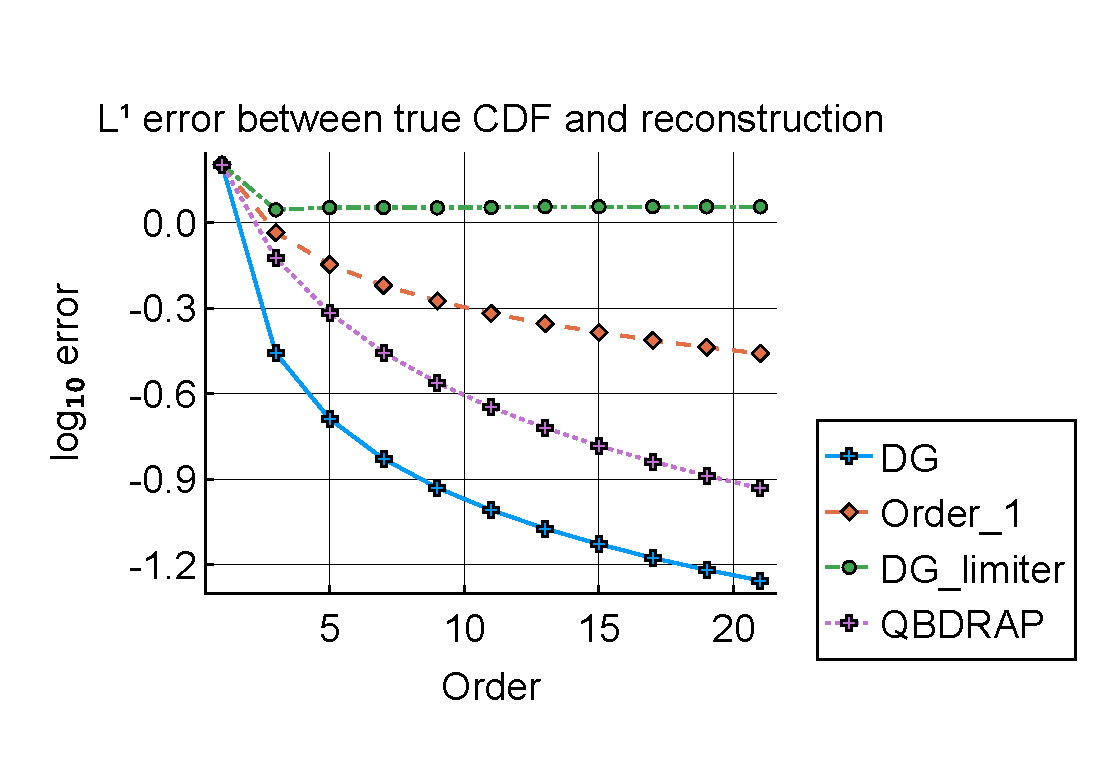
\includegraphics[width=0.5\textwidth,trim={0.75cm 0.8cm 0.25cm 1.25cm},clip]{chapter6/figs/wave/fun2/meshs_l1_cdf_error_formatted.pdf}%
	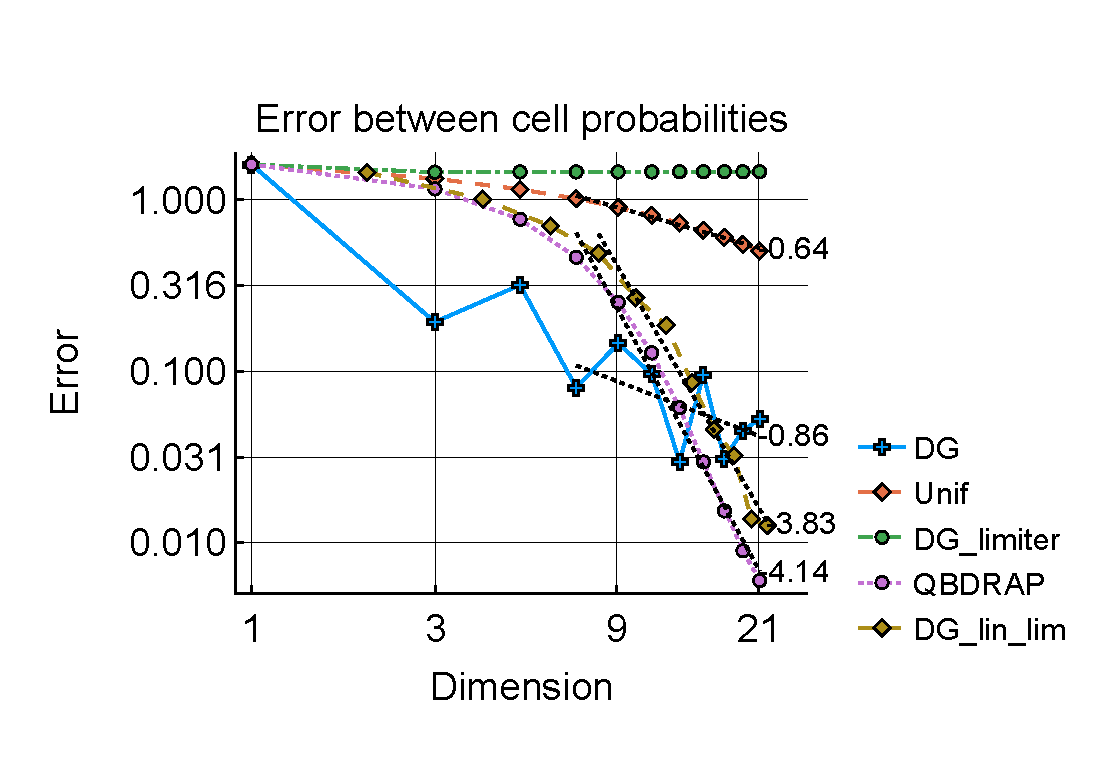
\includegraphics[width=0.5\textwidth,trim={0.75cm 0.8cm 0.25cm 1.25cm},clip]{chapter6/figs/wave/fun2/L1_cell_probs.pdf}
	\caption{\(L^1\) error between the true CDF, \(1(4.5\leq x)\), and the approximations (left) and the error metric based on the cell masses as described in (\ref{eqn: cell errors}) for the DG method (blue solid line with crosses), DG method with the MUSCL limiter (green dash-dotted line with crosses), uniformisation method (orange dashed line with diamonds) and QBD-RAP method (green dash-dotted line with circles).} 
	\label{fig: fun 2 wave} 
\end{figure}
\end{example}

\begin{example}
	Now consider an initial distribution which is truncated Gaussian with mean parameter 2.5 and standard deviation parameter 0.5, and trucated at the boundaries, 0 and 10;
	\begin{align}
		\mu([0,x)) := \mathbb P(X(0)\leq x, \varphi(0)=1)=\cfrac{\Phi((x-2.5)/0.5)1(0 \leq x < 10.0)}{\Phi(7.5/0.5)-\Phi(-2.5/0.5)} + 1(10\leq x), \label{eqn: kdjfksdf}
	\end{align}
	where \(\Phi(x)\) is the CDF of the standard normal distribution.

	Hence, at time \(t=4\) the distribution is truncated Gaussian with mean parameter 6.5, standard deviation parameter 0.5, and is truncated below at 4.0 and above at 10, and there is also a small mass at the upper boundary; 
	\begin{align}
		&\mathbb P(X(4)\leq x, \varphi(4)=1\mid X(0)\sim\mu, \varphi(0)=1) \nonumber 
		\\&=\cfrac{\Phi((x-6.5)/0.5)1(4.0\leq x)}{\Phi(7.5/0.5)-\Phi(-2.5/0.5)} + 1(10 \leq x)\label{eqn: bbbbbaabbaa}%\cfrac{\Phi(7.5/0.5)-\Phi(3.5/0.5)}{\Phi(7.5/0.5)-\Phi(-2.5/0.5)}.
	\end{align}
	The mass at the boundary is approximately \(1.28\times 10^{-12}\). There is a small discontinuity at \(x=4\) where the CDF jumps from \(0\) to \(\approx 2.87\times 10^{-7}\), due to the truncation of the initial distribution at \(0\). 

	Since the discontinuity at \(x=4\) is small (much smaller than numerical integration errors in the evaluation of the error metrics), and the distribution is otherwise smooth, we expect that the DG method will perform well for this example. Figure~\ref{fig: fun 6 wave} confirms that this is indeed the case. For both metrics the error obtained by the DG method rapidly decreases to a point where it is swamped by other numerical errors. This is charaterisitc of the DG method for smooth problems. For low order DG schemes there are regions where the approximated PDF is negative, however, as the order of the DG scheme increases, these regions dissipate. Interestingly, even though this is a relatively smooth problem, the DG method with MUSCL limiter does not perform well. It must be that the initial and transient distributions are sufficiently `pointy' that small oscillations in the numerical solutions occur, and the limiter reduces the order of the scheme to linear. Both the uniformisation and QBD-RAP schemes perform similarly to previous examples. 
	\begin{figure}
		\centering
		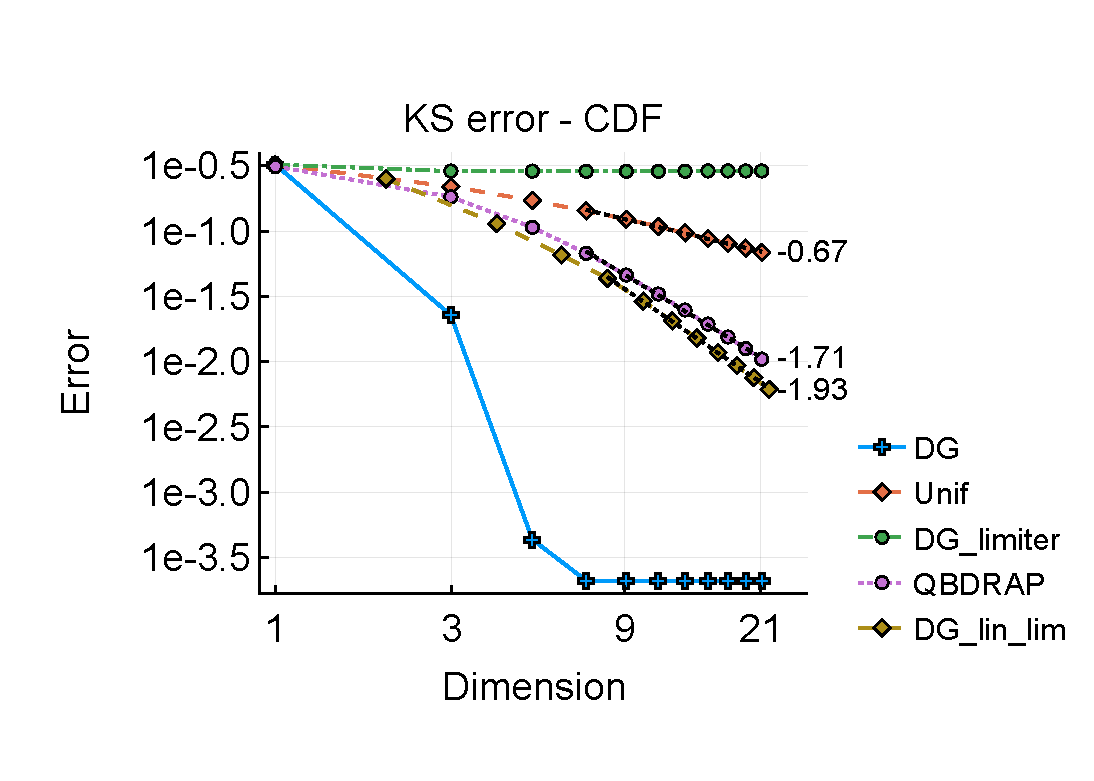
\includegraphics[width=0.5\textwidth,trim={0.75cm 0.8cm 0.25cm 1.25cm},clip]{chapter6/figs/wave/fun6/meshs_ks_error_formatted.pdf}%
		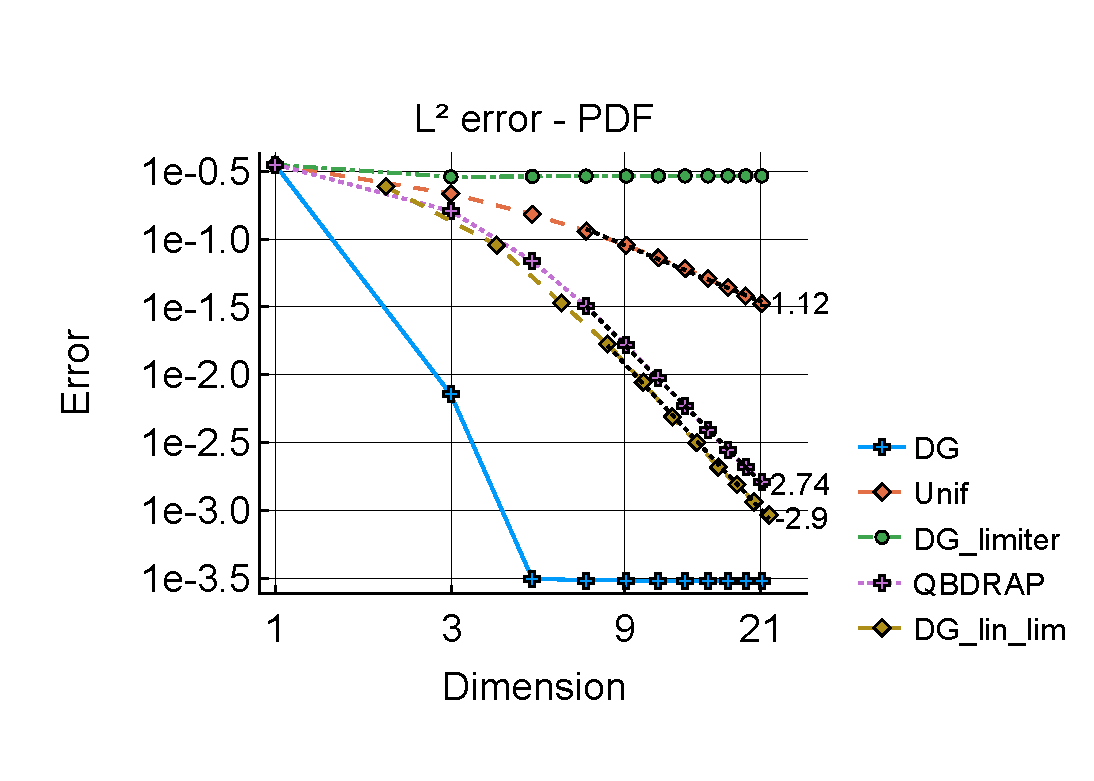
\includegraphics[width=0.5\textwidth,trim={0.75cm 0.8cm 0.25cm 1.25cm},clip]{chapter6/figs/wave/fun6/meshs_l2_pdf_error_formatted.pdf}
		\caption{KS error between the true CDF (Equation (\ref{eqn: bbbbbaabbaa})) and the approximations (left) and \(L^2\) error between the true PDF and the approximations for the DG method (blue solid line with crosses), DG method with the MUSCL limiter (green dash-dotted line with crosses), uniformisation method (orange dashed line with diamonds) and QBD-RAP method (green dash-dotted line with circles).} 
		\label{fig: fun 6 wave} 
	\end{figure}
\end{example}

\begin{example}
	We now want to look at how the methods might handle a point mass. We introduce an ephemeral second phase into the model with phase transition rate \(T_{22}=-1\), and fluid rate \(c_2=0\). The generator is therefore 
	\[T=\left[\begin{array}{cc} 0 & 0 \\ 1 & -1 \end{array}\right].\]

	We suppose that the initial condition is a point mass at the boundary in phase \(2\), i.e.~
	\[\mathbb P(X(0)\leq x, \varphi(0)=2)=1(0\leq x).\] 
	With this inital condition, the transient distribution at time \(t=4\) is 
	\begin{align}
		&\mathbb P(X(4)\leq x,\varphi(4)=1 \mid X(0)=0,\varphi(0)=2) \nonumber 
		\\&= e^{T_{22}4}\left(e^{-T_{22}x}-1\right)1(4< x) + (1-e^{T_{22}4})1(4\leq x) \nonumber
		\\&= e^{-4}\left(e^{4x}-1\right)1(4< x) + (1-e^{-4})1(4\leq x) \label{eqn: asjda}
	\end{align}
	and 
	\begin{align}
		\mathbb P(X(4)\leq x,\varphi(4)=2 \mid X(0)=0,\varphi(0)=2) = e^{-4}1(0\leq x).
	\end{align}
	The PDF at \(t=4\) is discontinuous at \(x=4\). For this problem, all methods can represent the initial condition exactly. 

	Figure~\ref{fig: fun 1 wave} plots the KS error metric between the true and approximated CDFs (right) and the \(L^2\) error metrics between the true and approximated PDFs. Observing Figure~\ref{fig: fun 1 wave}, as expected, since the solution is discontinuous, the DG method with MUSCL limiter does perform well. The uniformisation and QBD-RAP methods appear to converge, with the QBD-RAP method converging faster. DG method converges fastest, however, produces approximations with negative and oscillatory solutions as we might expect given the discontinuity. A selection of approximations to the transient PDF are shown in Figure~\ref{fig: pdf wave fun 1}
	\begin{figure}
		\centering
		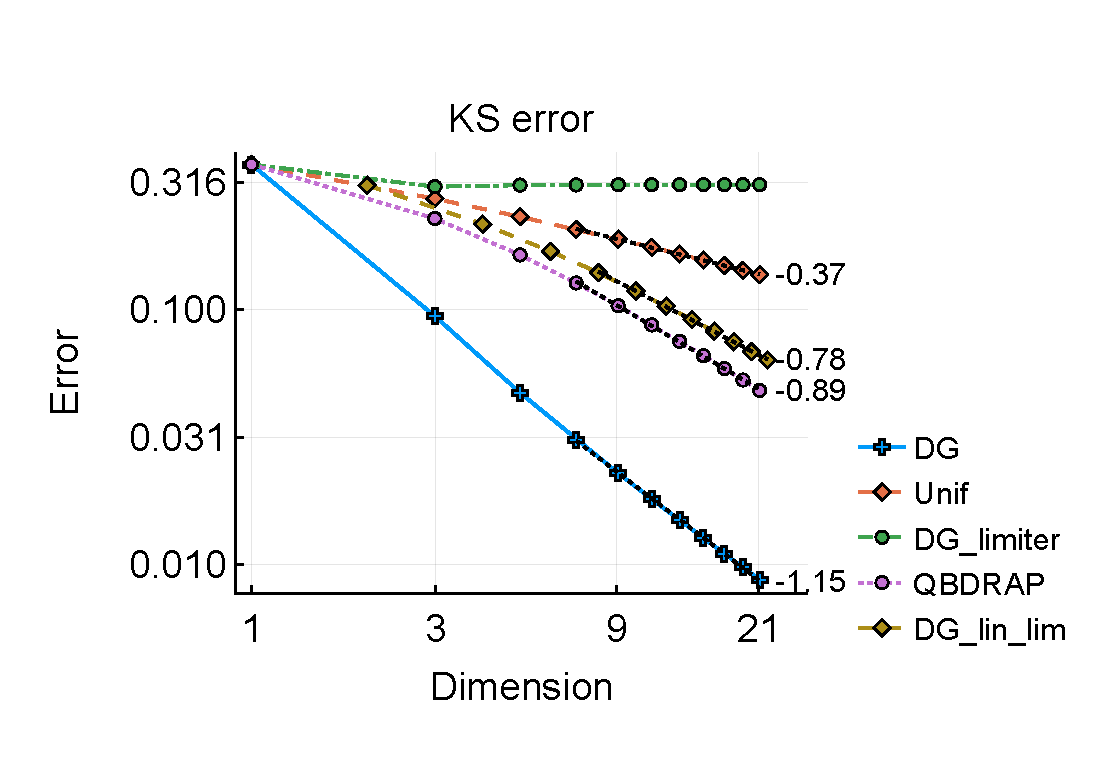
\includegraphics[width=0.5\textwidth,trim={0.75cm 0.8cm 0.25cm 1.25cm},clip]{chapter6/figs/wave/fun1/meshs_ks_error_formatted.pdf}%
		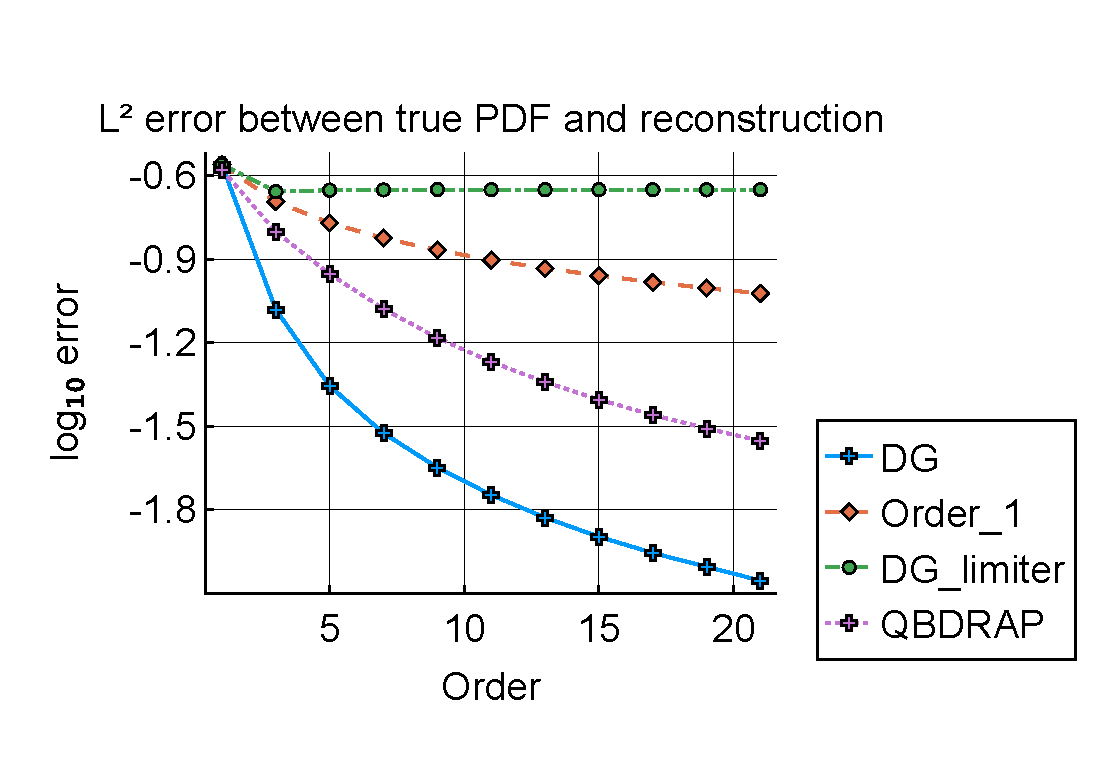
\includegraphics[width=0.5\textwidth,trim={0.75cm 0.8cm 0.25cm 1.25cm},clip]{chapter6/figs/wave/fun1/meshs_l2_pdf_error_formatted.pdf}
		\caption{KS error between the true CDF (Equation (\ref{eqn: asjda})) and the approximations (left) and \(L^2\) error between the true PDF and the approximations for the DG method (blue solid line with crosses), DG method with the MUSCL limiter (green dash-dotted line with crosses), uniformisation method (orange dashed line with diamonds) and QBD-RAP method (green dash-dotted line with circles).} 
		\label{fig: fun 1 wave} 
	\end{figure}
	\begin{figure}
		\centering
		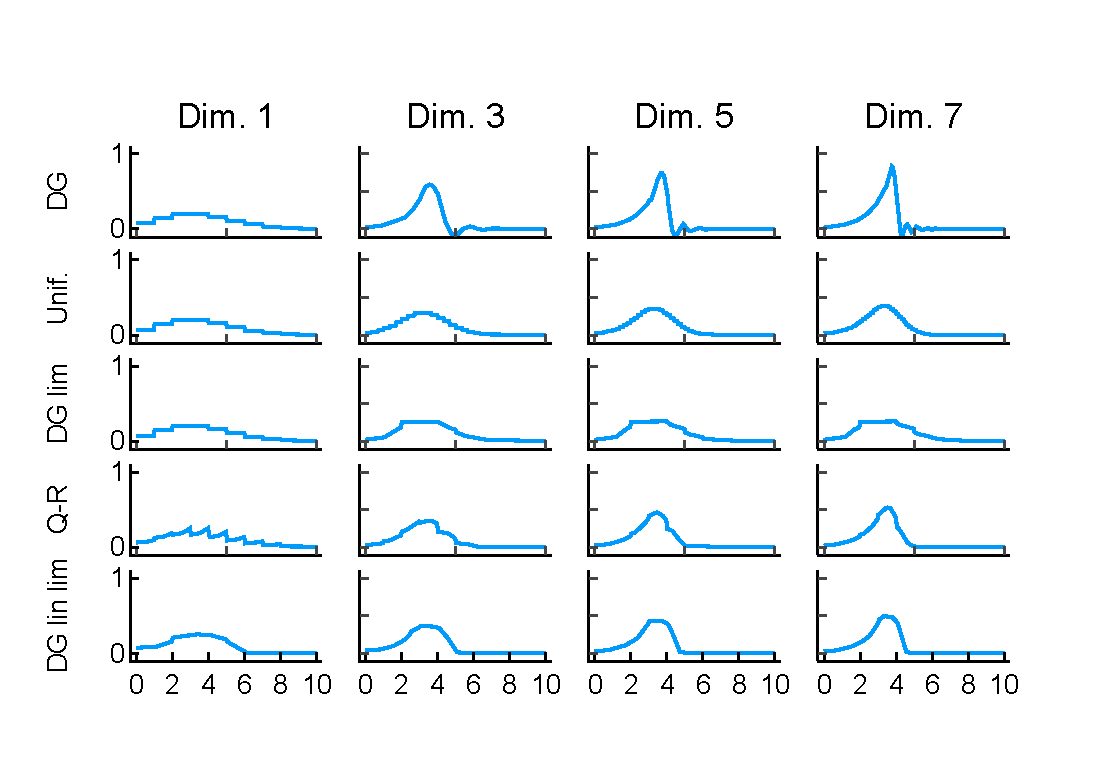
\includegraphics[width=\textwidth]{chapter6/figs/wave/fun1/pdf_formatted.pdf}
		\caption{Reconstructed PDFs using the DG (top row), uniformisation (second row), DG with MUSCL limiter (third row) and QBD-RAP (bottom row) methods, for order 1, 3, 5, and 7 (columns). The true density function is \(e^{-4}e^{x}1(x<4)\).} 
		\label{fig: pdf wave fun 1}
	\end{figure} 
\end{example} 

\FloatBarrier

\section{Stationary distributions} \label{sec:stat}
We briefly turn our attention to stationary distributions of fluid queue. Since the stationary distribution is smooth, apart from at the boundaries, we expect that the DG method will work well here. The stationary distributions are conveninent as they can be evaluated analytically (CITE) and do not require us to approximate initial conditions or integrate over time.

Here we analyse two simple models which are based on Example~2 in \citep{bean2009}, except here we introduce add a lower boundary to the model (no lower boundary is specified in Example~2 of \citep{bean2009} as it is inconsequential to their analysis). 

\begin{model}\label{model: simple}
	Consider a fluid queue where the driving process is a CTMC with state space \(\calS=\{1,2,3,4\}\), generator 
	\[\bs T = \left[\begin{array}{cccc}
		-1.1 & 1.1 & 0 & 0 \\
		1 & -1 & 0 & 0 \\ 
		0.01 & 0 & -0.01 & 0 \\
		0 & 0.01 & 0 & -0.01 
	\end{array}\right],\]
	and there are associated rates \(c_1=1, c_2 = -1, c_3=0, c_4=0\) and boundaries at \(x=0\) and \(x=10\). We specify two types of behaviour at the boundary.
	\begin{enumerate}[a)]
		\item (Absorbing model) Upon hitting the lower boundary, the process transitions from phase \(2\) to phase \(j\) with probability \(p_{2j}\) where 
		\[\vligne{p_{21} & p_{22} & p_{23} & p_{24}} = \vligne{0 & 0 & 1 & 0}.\]
		Upon hitting the upper boundary, the process transitions from phase \(1\) to phase \(j\) with probability \(p_{1j}\) where 
		\[\vligne{p_{11} & p_{12} & p_{13} & p_{14}} = \vligne{0 & 0 & 0 & 1}.\]
		\item (Reflecting model) Upon hitting the lower boundary, the process transitions from phase \(2\) to phase \(j\) with probability \(p_{2j}\) where 
		\[\vligne{p_{21} & p_{22} & p_{23} & p_{24}} = \vligne{1 & 0 & 0 & 0}.\]
		Upon hitting the upper boundary, the process transitions from phase \(1\) to phase \(j\) with probability \(p_{1j}\) where 
		\[\vligne{p_{11} & p_{12} & p_{13} & p_{14}} = \vligne{0 & 1 & 0 & 0}.\]
	\end{enumerate}
\end{model}
Phases~3 and 4 are included only to capture behaviour at the boundary.

For Model~\ref{model: simple}~a), upon hitting the boundary, the process stays at the boundary for an exponentially distributed amount of time with mean 100. For Model~\ref{model: simple}~b), upon hitting the boundary, the process is immediately reflected. In Model~\ref{model: simple}~b) phases 3 and 4 are ephemeral and are included only for notational convenience. 

The models were discretised using the DG, uniformisation and QBD-RAP methods using ten cells of width \(1\). We compute the coefficients for the stationary distribution in the following way. Suppose that a given discretisation method results in an approximation to the generator of the fluid queue as a matrix \(\bs B\). Then the stationary coefficients are found by solving 
\begin{align}
	\bs b \bs B = 0,\\
	\mbox{such that } \bs b\bs 1=1,
\end{align}
for the coefficients \(\bs b\). 

\paragraph{Model~\ref{model: simple}~a) Absorbing model}
Figure~\ref{fig: absorbing stationary} plots KS errors between the true stationary CDF and the approximations (left) and the \(L^2\) error between the true stationary PDF and the approximations. Clearly the DG method is superior here as its error rapidly decrease to a point where is become insignificant compared to other numerical errors. The QBD-RAP method and uniformisation method both appear to be converging, with the errors for the QBD-RAP method decreasing faster.
\begin{figure}
	\centering
	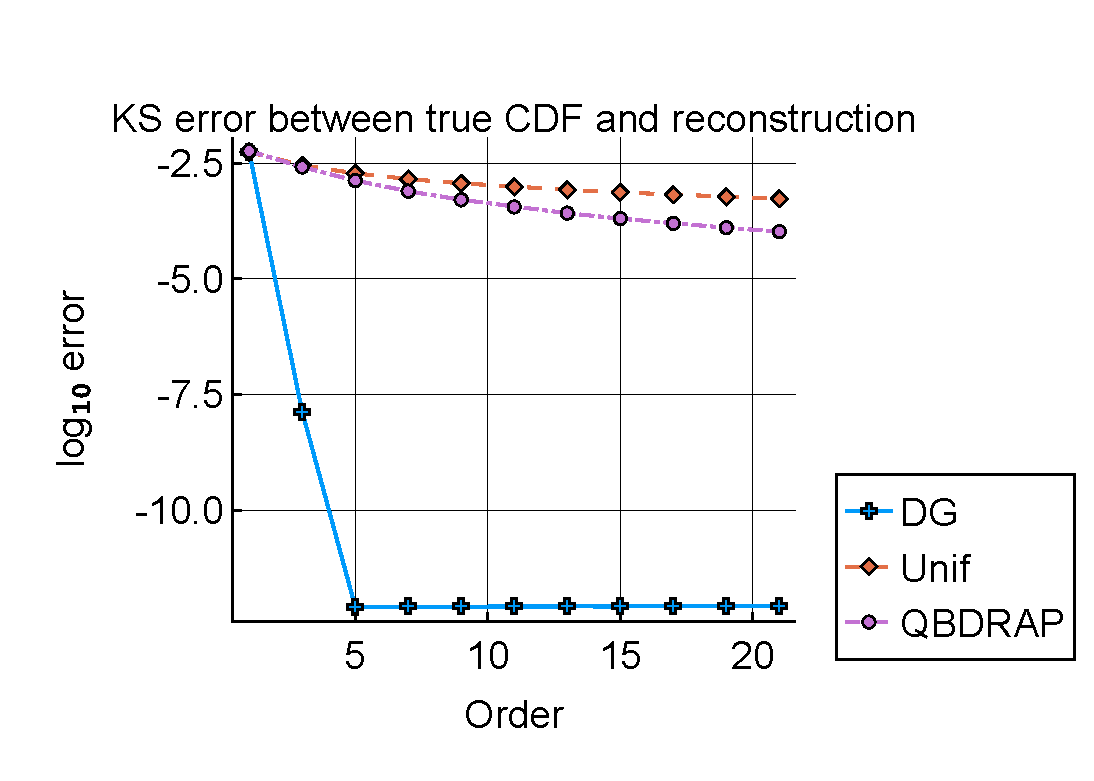
\includegraphics[width=0.5\textwidth,trim={0.75cm 0.8cm 0.25cm 1.25cm},clip]{chapter6/figs/hitting_times_model/absorbing_model/stationary_distribution/ks_error_formatted.pdf}%
	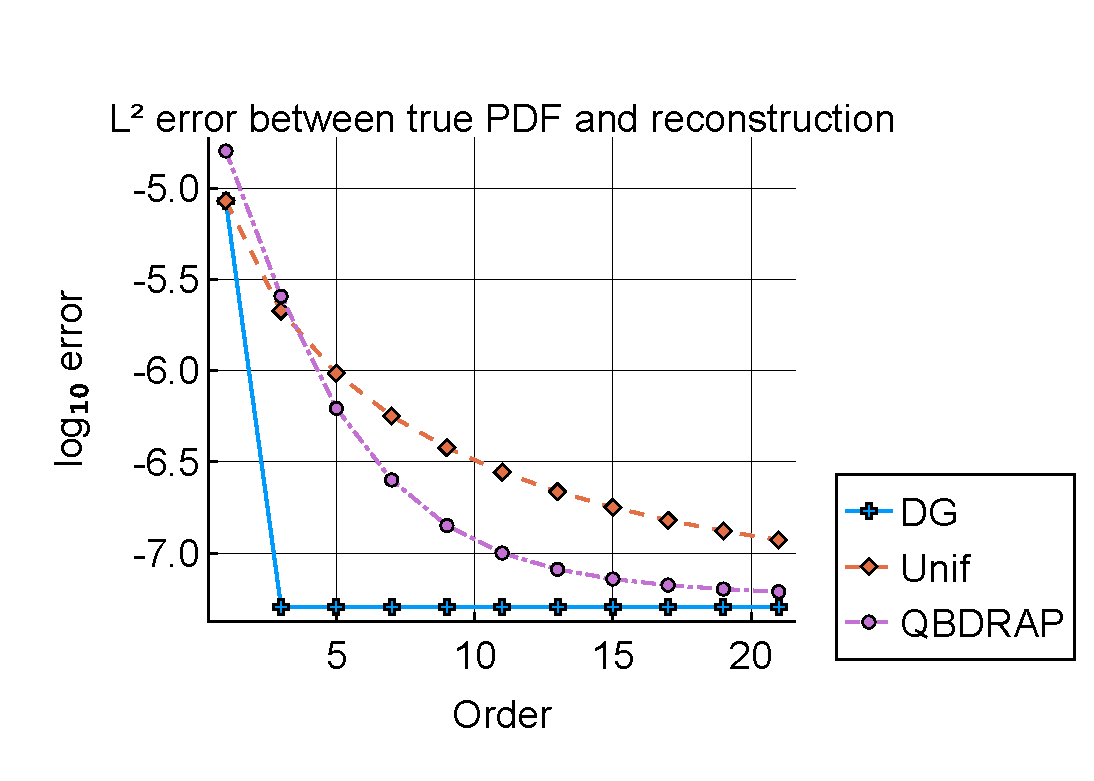
\includegraphics[width=0.5\textwidth,trim={0.75cm 0.8cm 0.25cm 1.25cm},clip]{chapter6/figs/hitting_times_model/absorbing_model/stationary_distribution/l2_pdf_error_formatted.pdf}
	\caption{KS error between the true stationary CDF  and the approximations (left) and \(L^2\) error between the true stationary PDF and the approximations for Model~\ref{model: simple}~a) using the DG method (blue solid line with crosses), uniformisation method (orange dashed line with diamonds) and QBD-RAP method (green dash-dotted line with circles).} 
	\label{fig: absorbing stationary} 
\end{figure}

\paragraph{Model~\ref{model: simple}~b) Reflecting model}
Figure~\ref{fig: reflecting stationary} plots KS errors between the true stationary CDF and the approximations (left) and the \(L^2\) error between the true stationary PDF and the approximations. Once again, the DG method is superior, the QBD-RAP method and uniformisation method both appear to be converging, with the errors for the QBD-RAP method decreasing faster.
\begin{figure}
	\centering
	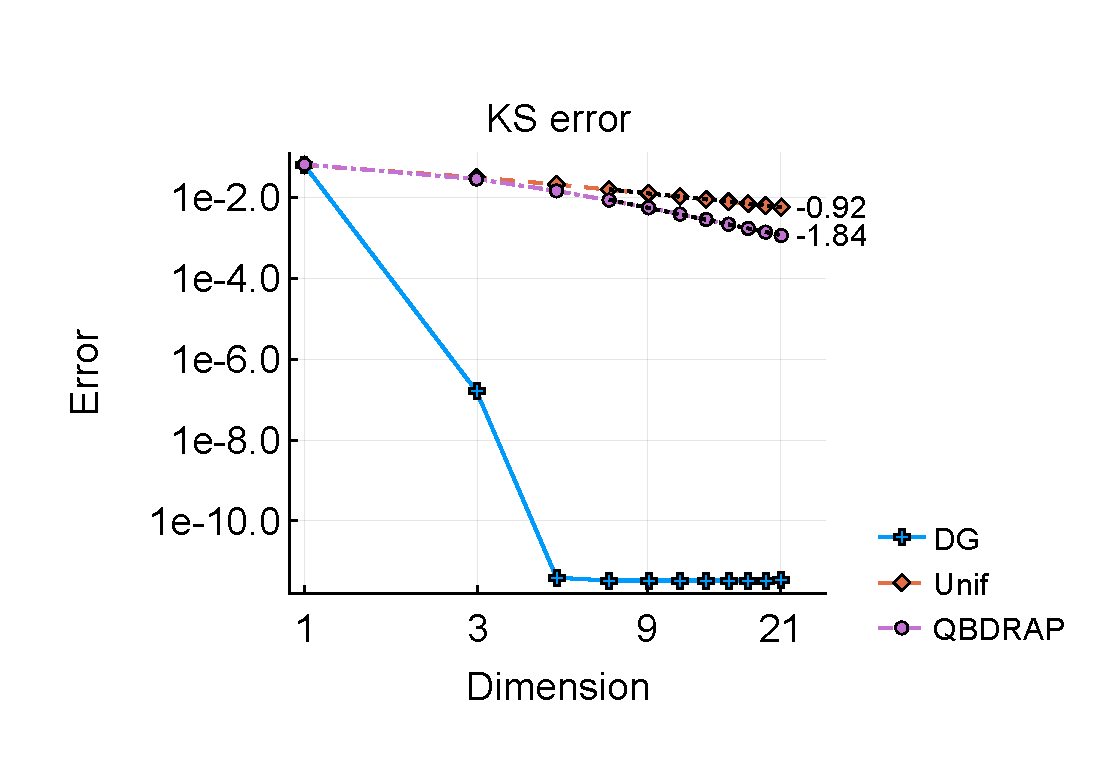
\includegraphics[width=0.5\textwidth,trim={0.75cm 0.8cm 0.25cm 1.25cm},clip]{chapter6/figs/hitting_times_model/reflecting_model/stationary_distribution/ks_error_formatted.pdf}%
	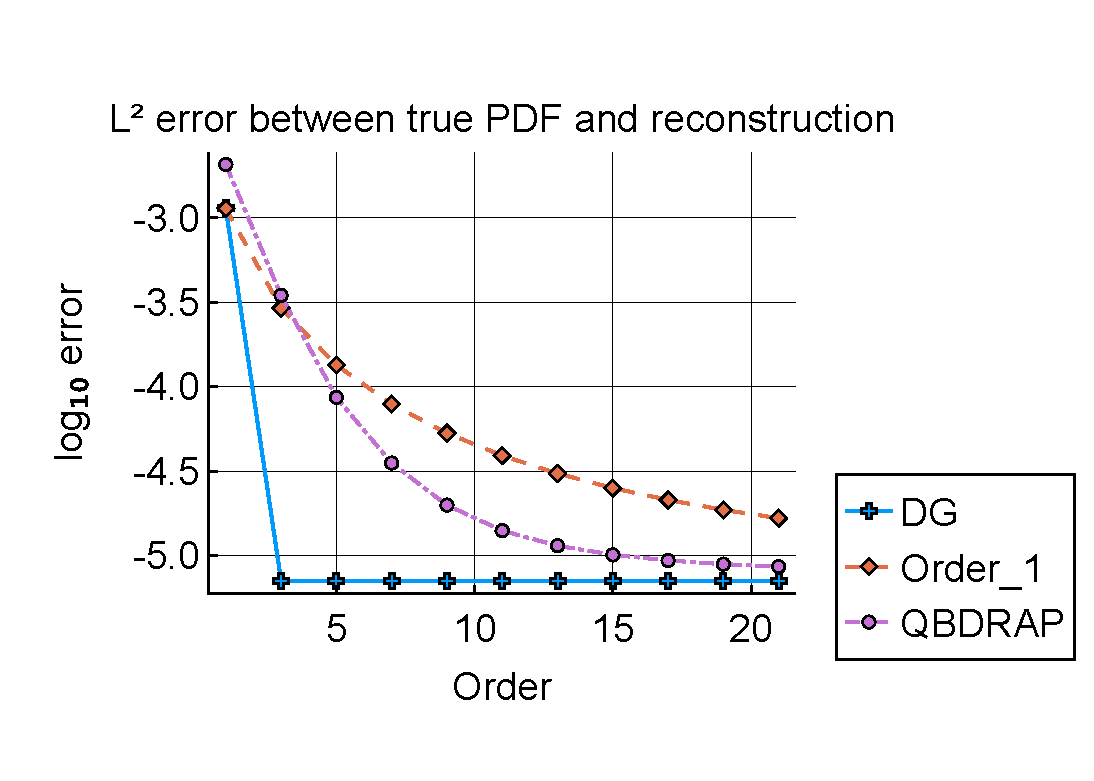
\includegraphics[width=0.5\textwidth,trim={0.75cm 0.8cm 0.25cm 1.25cm},clip]{chapter6/figs/hitting_times_model/reflecting_model/stationary_distribution/l2_pdf_error_formatted.pdf}
	\caption{KS error between the true stationary CDF and the approximations (left) and \(L^2\) error between the true stationary PDF and the approximations for Model~\ref{model: simple}~b) using the DG method (blue solid line with crosses), uniformisation method (orange dashed line with diamonds) and QBD-RAP method (green dash-dotted line with circles).} 
	\label{fig: reflecting stationary} 
\end{figure}

\section{Transient distributions}
Once again we consider Model~\ref{model: simple}~b)\footnote{We do not include the results for Model~\ref{model: simple}~a) as, for the purposes of the comparisons here, they are much the same as those reported for Model~\ref{model: simple}~b)} and use the same spatial discretisation as described in Section~\ref{sec:stat} (ten cells with width \(\Delta=1\)). Two initial conditions are considered, a point mass at 0.0 in phase 1, and the initial distribution with PDF 
\begin{align}
	\cfrac{1}{2}e^{-x}/(1-e^{-10})\label{eqn: exp init cond}
\end{align}
in phases 1 and 2, with no mass at the boundaries. We numerically integrate over time until time \(t=2.0\) using the SSPRK4 method with t-step size 0.005. We apply the DG method with, and without, the Generalised MUSCL slope limiter. 

To obtain a \emph{ground truth} 5,000,000 realisations of the fluid queue were simulated until \(t=2\), then the empirical CDF and the mass within each cell and at the boundaries were computed from the simulations. We do not attempt to numerically approximate the true PDF via simulation. We then compute the KS and \(L^1\) error metrics between the approximated CDF and simulated CDF, as well as the cell-wise error metric, given as follows. 
\begin{align}
	&\sum_{j\in\{1,2\}}\sum_{\ell=1}^{10} \left|\mathbb P(X(2)\in\calD_{\ell,j}, \varphi(2)=j\mid X(0)=0.5,\varphi(0)=1)-p(2,\ell,j)\right|\nonumber 
	\\&+\left|\mathbb P(X(2)\in\{10\}, \varphi(2)=4\mid X(0),\varphi(0))-p(2,11,4)\right|\nonumber 
	\\&+\left|\mathbb P(X(2)\in\{0\}, \varphi(2)=3\mid X(0),\varphi(0))-p(2,0,3)\right| \label{eqn: cell errors 2}
\end{align}
where \(p(2,\ell,j)\) is an approximation to \(\mathbb P(X(2)\in\calD_{\ell,j}, \varphi(2)=j\mid X(0),\varphi(0))\), \(p(2,11,4)\) is an approximation to \(\mathbb P(X(2)\in\{10\}, \varphi(2)=4\mid X(0),\varphi(0))\), and \(p(2,0,3)\) is an approximation to \(\mathbb P(X(2)\in\{10\}, \varphi(2)=3\mid X(0),\varphi(0))\). 

To account for possible Monte-Carlo error, we used a bootstrap with 1,000 bootstrap samples. That is, we sample, with replacement, 5,000,000 realisations of the fluid queue from the original 5,000,000 samples, then compute error metrics with the resampled data. We resample 1,000 times. Via the bootstrap, we report the \(5\)th and \(95\)th percentile of the sampling distribution of the errors. 

To evaluate error metrics, we use a grid of 10,001 evenly spaced points for each phase. 

To approximate the point mass initial condition we compute the initial coefficients for each scheme exactly. For the exponential initial condition (\ref{eqn: exp init cond}) we compute the initial coefficients via Gauss-Lobatto quadrature for the DG method, by using the mid-point rule for the uniformisation method, and by using a trapezoidal rule with 2,001 points on each cell for the QBD-RAP method. 

\paragraph{Model~\ref{model: simple}~b) Reflecting model with exponential initial condition}
Figure~\ref{fig: reflecting transient exp} shows the error metrics for the four different spatial discretisation schemes (DG, DG with MUSCL limiter, uniformisation and QBD-RAP). For both error metrics the DG scheme converges rapidly until computational errors become significant. The uniformisation and QBD-RAP schemes converge at a slower rate, with the QBD-RAP scheme converging at a faster rate. The DG scheme with MUSCL limiter does not appear to be converging, which suggests there is at least one iteration during the numerical integration over time at which the numerical solution displays oscillations. However, when the DG approximations for the distribution at time \(t=2\) are plotted, they do not display oscillations. This suggests that the oscillations which might occur with the DG scheme must be transient, and have dissipated by time \(t=2\).%
\begin{figure}
	\centering
	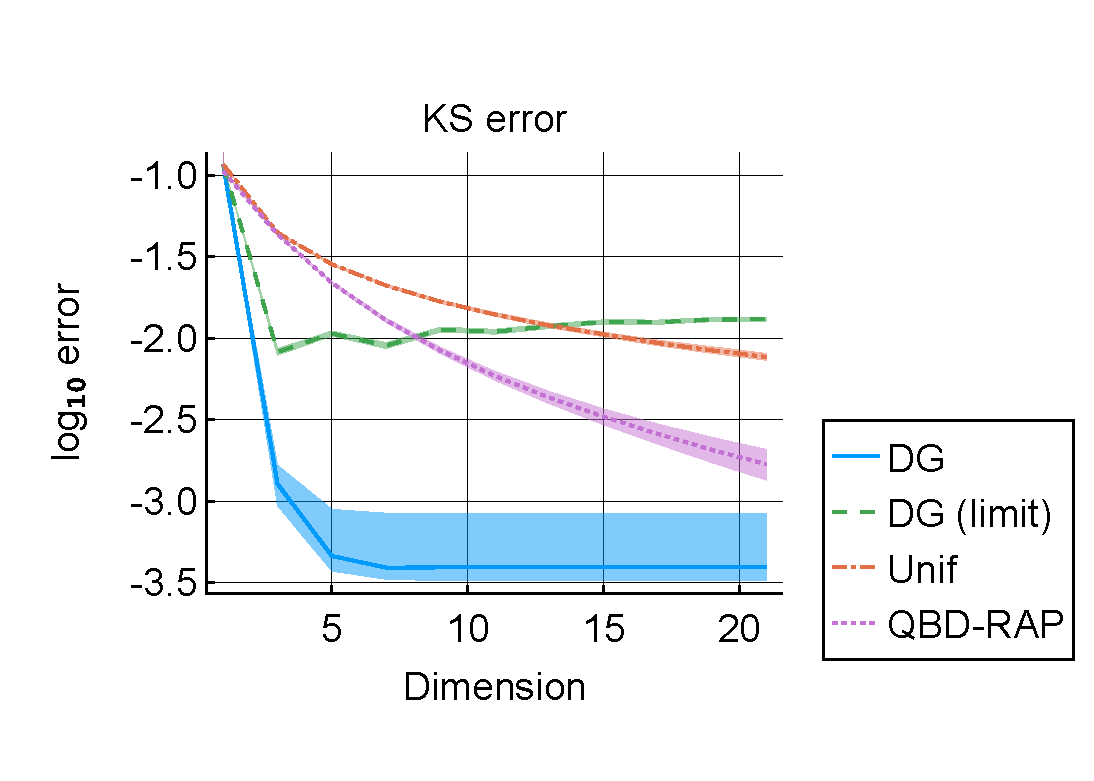
\includegraphics[width=0.5\textwidth,trim={0.75cm 0.8cm 0.25cm 1.25cm},clip]{chapter6/figs/hitting_times_model/reflecting_model/transient_distribution/exp/ks_error_formatted.pdf}%
	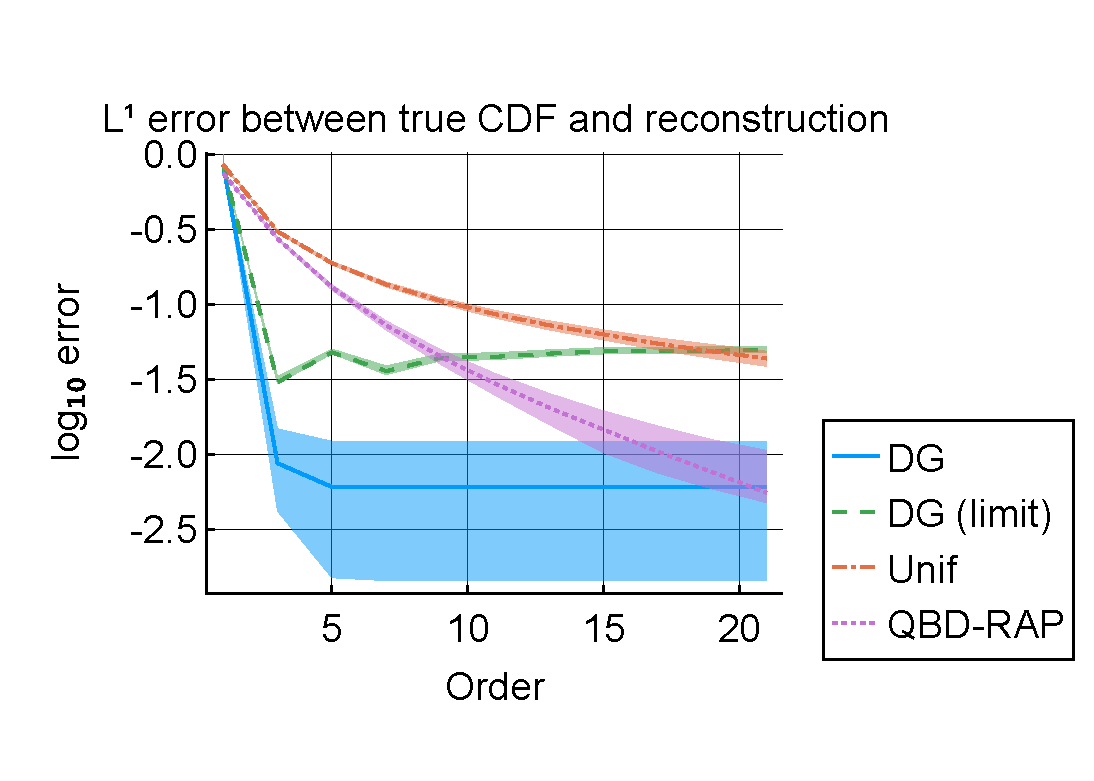
\includegraphics[width=0.5\textwidth,trim={0.75cm 0.8cm 0.25cm 1.25cm},clip]{chapter6/figs/hitting_times_model/reflecting_model/transient_distribution/exp/l1_cdf_error_formatted.pdf}
	\caption{KS (left) and \(L^1\) (right) errors between the true transient CDF at time \(t=2\) for Model~\ref{model: simple}~b) with the exponential initial condition, and the corresponding approximations obtained via the DG method (blue solid line), DG method with Generalised MUSCL limiter (green dashed line), uniformisation method (orange dashed line) and QBD-RAP method (purple dotted line).} 
	\label{fig: reflecting transient exp} 
\end{figure}

\paragraph{Model~\ref{model: simple}~b) Reflecting model with a point-mass initial condition}
Figure~\ref{fig: reflecting transient pm} shows the error metrics for the four different spatial discretisation schemes (DG, DG with MUSCL limiter, uniformisation and QBD-RAP). Comparing the error metrics in Figure~\ref{fig: reflecting transient pm} for the point mass initial condition, with the ones in Figure~\ref{fig: reflecting transient exp} for the exponential initial condition, all schemes perform worse for the point mass initial condition. Regarding comparative rates of convergence, we come to similar conclusions as we did for the exponential initial condition. The DG scheme converges fastest, followed by the QBD-RAP scheme, then the uniformisation scheme, while the DG scheme with MUSCL limiter does not appear to converge due to the limiter reducing the scheme to a linear approximation in the spatial variable. %
\begin{figure}
	\centering
	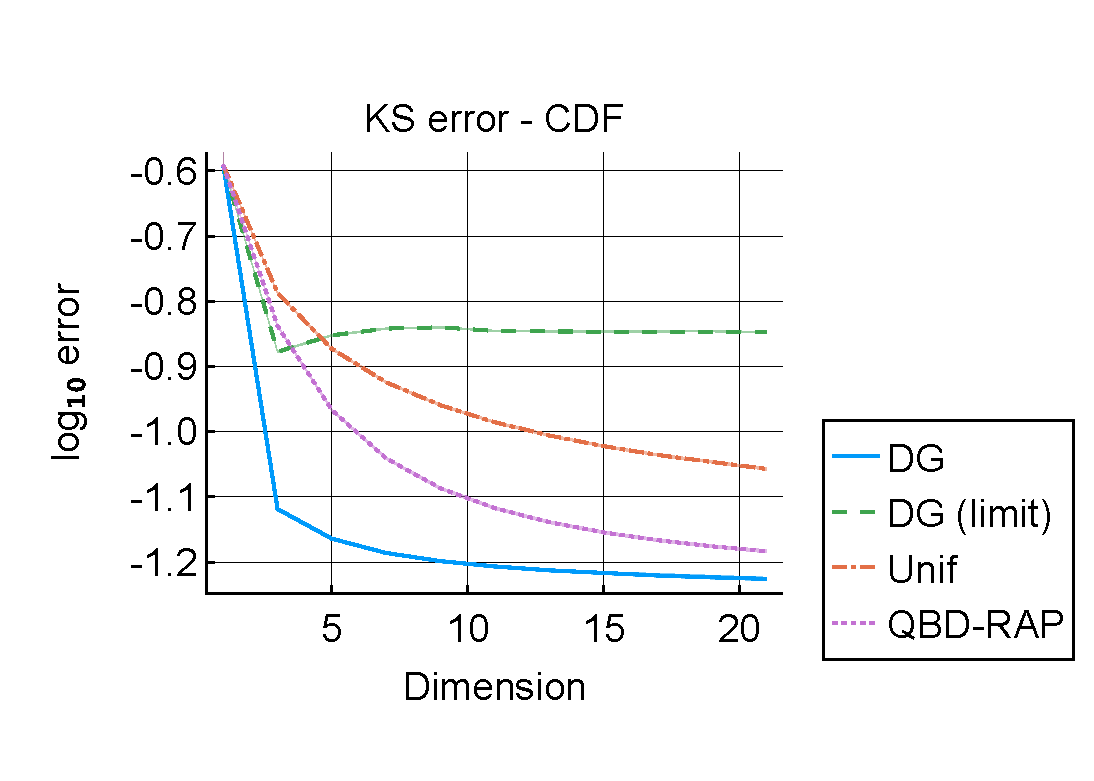
\includegraphics[width=0.5\textwidth,trim={0.75cm 0.8cm 0.25cm 1.25cm},clip]{chapter6/figs/hitting_times_model/reflecting_model/transient_distribution/point_mass/ks_error_formatted.pdf}%
	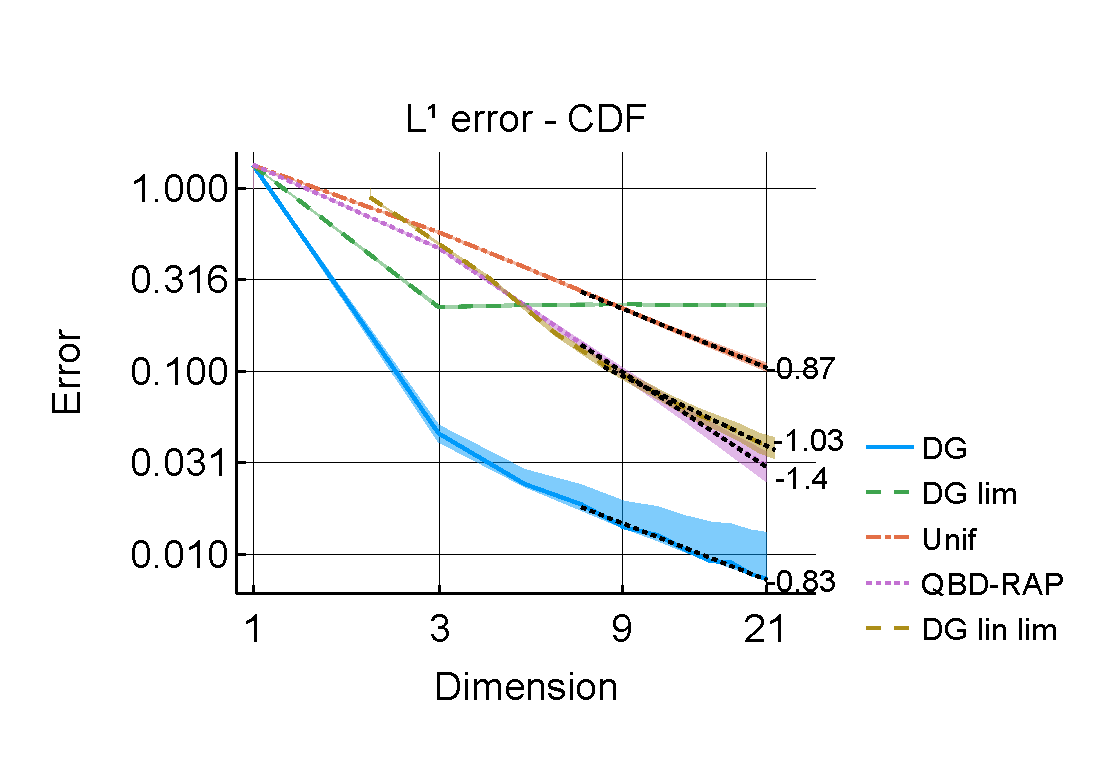
\includegraphics[width=0.5\textwidth,trim={0.75cm 0.8cm 0.25cm 1.25cm},clip]{chapter6/figs/hitting_times_model/reflecting_model/transient_distribution/point_mass/l1_cdf_error_formatted.pdf}
	\caption{KS (left) and \(L^1\) (right) errors between the true transient CDF at time \(t=2\) for Model~\ref{model: simple}~b) with the point-mass initial condition, and the corresponding approximations obtained via the DG method (blue solid line), DG method with Generalised MUSCL limiter (green dashed line), uniformisation method (orange dashed line) and QBD-RAP method (purple dotted line).} 
	\label{fig: reflecting transient pm} 
\end{figure}
\FloatBarrier

\section{Hitting/Exit times}
\begin{model}\label{model: simple2}
Consider an unbounded fluid queue with two phases, generator 
\[\bs T = \left[\begin{array}{cc}
	-1.1 & 1.1 \\
	1 & -1
\end{array}\right],\]
and associated rates \(c_1=1, c_2=-1\). We approximate the first exit time of the interval \([0,1]\). 
\end{model}
Let \(\theta = \{\inf t>0 \mid X(t)=0, \mbox{ or }X(t)=1\},\) then the distribution of the exit time in phase \(i\in\{1,2\}\) is 
\begin{equation}\label{eqn: hit cdf}\mathbb P(\theta < t, \varphi(t)=i\mid \bs X(0)\sim \mu),\end{equation}
for some initial distribution \(\mu\). We look at two initial conditions; an exponential with equal mass in each phase, 
\[\mathbb P(X(0)\in\wrt x,\varphi(0)=i) = exp(-x)/(1-exp(-1))/2,\]
and a point mass at \(X(0)=0\) in phase \(\varphi(0)=1\). 

To do so, we partition \([0,1]\) into three intervals of width \(1/3\), and use the DG, uniformisation and QBD-RAP methods to discretise the fluid queue. To capture the mass which has left the interval \([0,1]\), we suppose that when the process hits the boundary it is absorbed forever at the boundary and remains in the phase which it hit the boundary. 

We integrate the discretisations until time \(t=10\) using the SSPRK4 method with t-step size 0.005. We use the DG scheme with and without a slope limiter during the time-integration. At each time-step of the numerical integration, we record the amount of mass at the absorbing boundaries in each phase, which gives us an approximation of the cumulative distribution function of the exit time in each phase up to time \(t=10\). 

For comparison, we simulated 5,000,000 realisations and recorded the exit time from the interval \([0,1]\) and the phase at the time of exit. We then compute the empirical CDF of the hitting probabilities 
\[\mathbb P(\theta < t, \varphi(t)=i\mid \bs X(0)\sim \mu),\] 
for \(t=0.005\times k\), \(k=0,...,2000\). 

To account for Monte-Carlo errors, we took 1,000 bootstrap resamples of the original 5,000,000 samples and computed the empirical CDF of the hitting probabilities for each bootstrap sample. For each bootstrap sample, we resampled 5,000,000 points. For each bootstrap sample we compute error metrics between the empirical and approximated CDFs and recorded the 5th and 95th percentile of the distribution of the errors. 

\paragraph{Exponential initial condition}
Figure~\ref{fig: hitting time exp} shows the error metrics recorded for the four different numerical approximation schemes. The uniformisation and QBD-RAP method both appear to converge, with the QBD-RAP converging at a faster rate. For both error metrics, the DG scheme converges rapidly to order 5, after which there is no further improvement. The DG scheme with MUSCL limiter does not appear to converge, suggesting oscillations in the DG approximation. However, there are no obvious signs of this oscillation in the exit-time CDF. For the KS-metric, the QBD-RAP scheme outperforms the DG scheme at orders 15, 17 and 21, which, to me, is unexpected. Perhaps the oscillations in the DG scheme are preventing more accurate solutions, or it could be that certain numerical errors in the QBD-RAP scheme have had a favourable cancellation and caused a lower error.
\begin{figure}
	\centering
	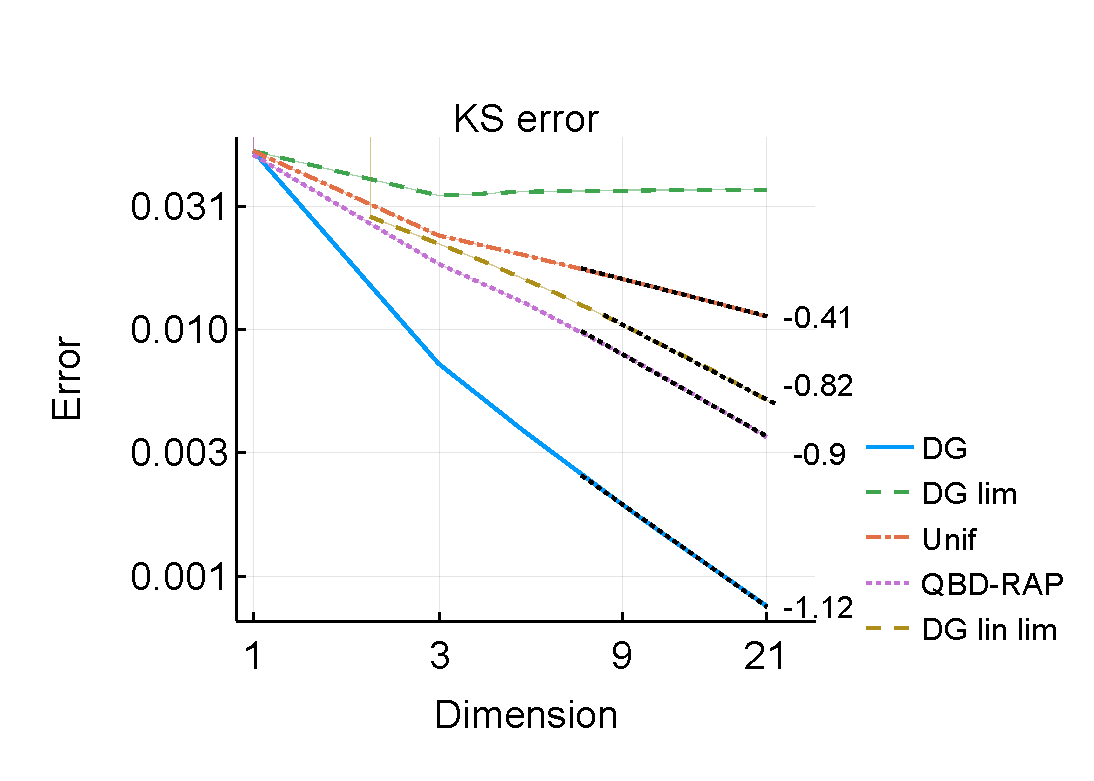
\includegraphics[width=0.5\textwidth,trim={0.75cm 0.8cm 0.25cm 1.25cm},clip]{chapter6/figs/hitting_times_model/hitting_times/exp/ks_error_formatted.pdf}%
	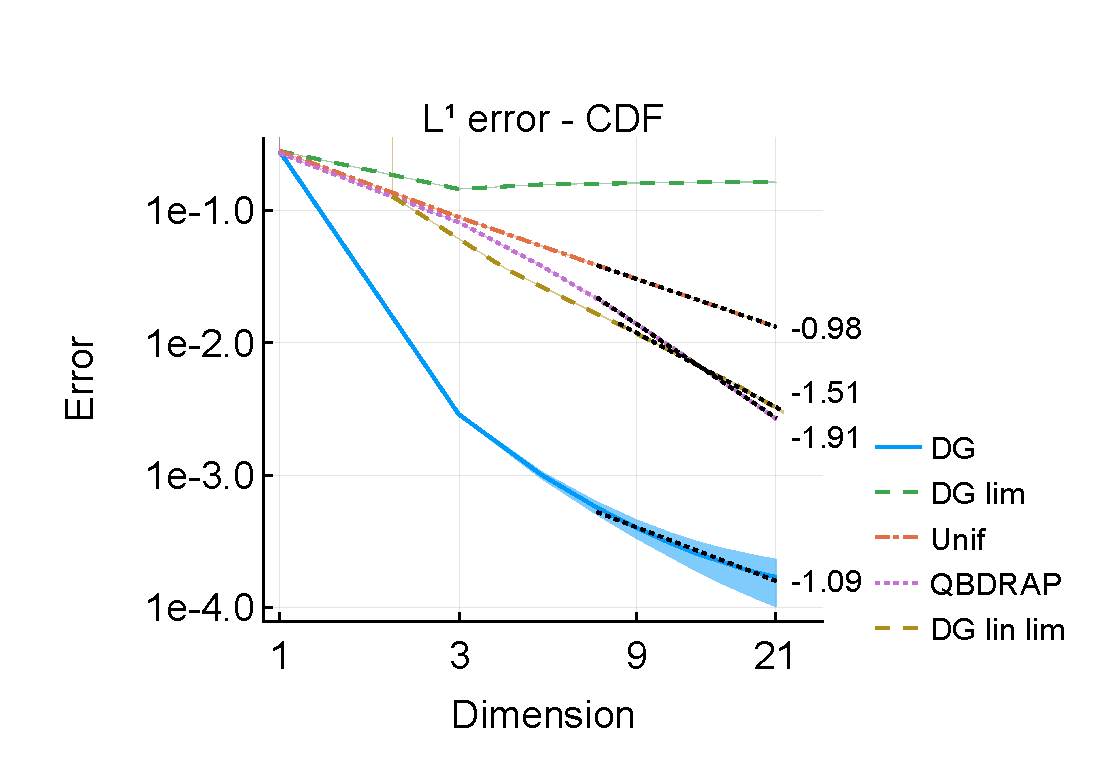
\includegraphics[width=0.5\textwidth,trim={0.75cm 0.8cm 0.25cm 1.25cm},clip]{chapter6/figs/hitting_times_model/hitting_times/exp/l1_cdf_error_formatted.pdf}
	\caption{KS (left) and \(L^1\) (right) errors between the simulated and approximated first exit time CDFs (Equation~\ref{eqn: hit cdf}) for Model~\ref{model: simple2} with the exponential initial condition. The approximations were obtained via the DG method (blue solid line), DG method with Generalised MUSCL limiter (orange dashed line), uniformisation method (green dashed line) and QBD-RAP method (purple dotted line). Bootstrapped 90\% confidence intervals are shown by the lighter coloured bars surrounding the lines.} 
	\label{fig: hitting time exp} 
\end{figure}

\paragraph{Point mass initial condition}
Figure~\ref{fig: hitting time pm} shows the error metrics recorded for the four different numerical approximation schemes. The uniformisation and QBD-RAP method both appear to converge, with the QBD-RAP converging at a faster rate. The DG scheme with MUSCL limiter does not appear to converge, suggesting oscillations in the DG approximation. The DG scheme appears to converge fastest up to the order-19 scheme, at which point the error increases. This is caused by oscillations in the numerical solution. In this case we can observe the oscillation in the exit time CDF. 

In Figure~\ref{fig: hitting time oscillation} we plot the CDFs of the exit time for phase 1, obtained via the DG scheme and QBD-RAP scheme, each using an order-21 basis, and also via simulation. Observing Figure~\ref{fig: hitting time oscillation} the DG approximation clearly displays oscillations around \(t=0\) and \(t=1\). The largest oscillations are around \(t=0\). 
\begin{figure}
	\centering
	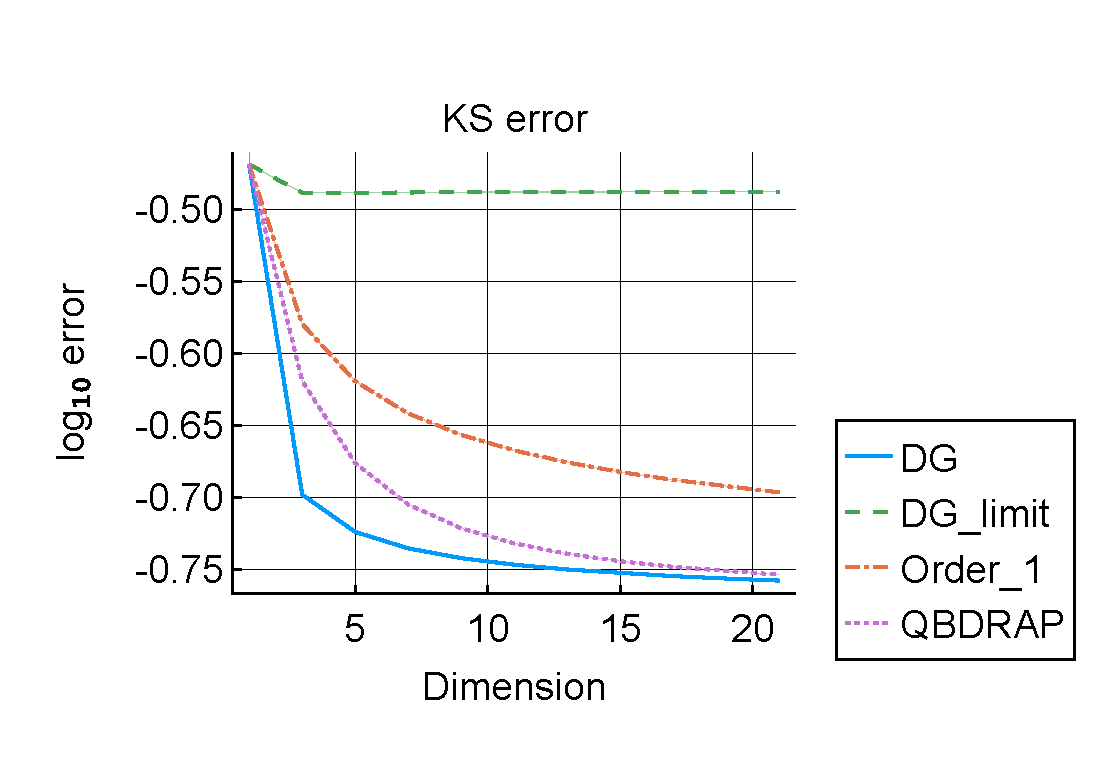
\includegraphics[width=0.5\textwidth,trim={0.75cm 0.8cm 0.25cm 1.25cm},clip]{chapter6/figs/hitting_times_model/hitting_times/point_mass/ks_error_formatted.pdf}%
	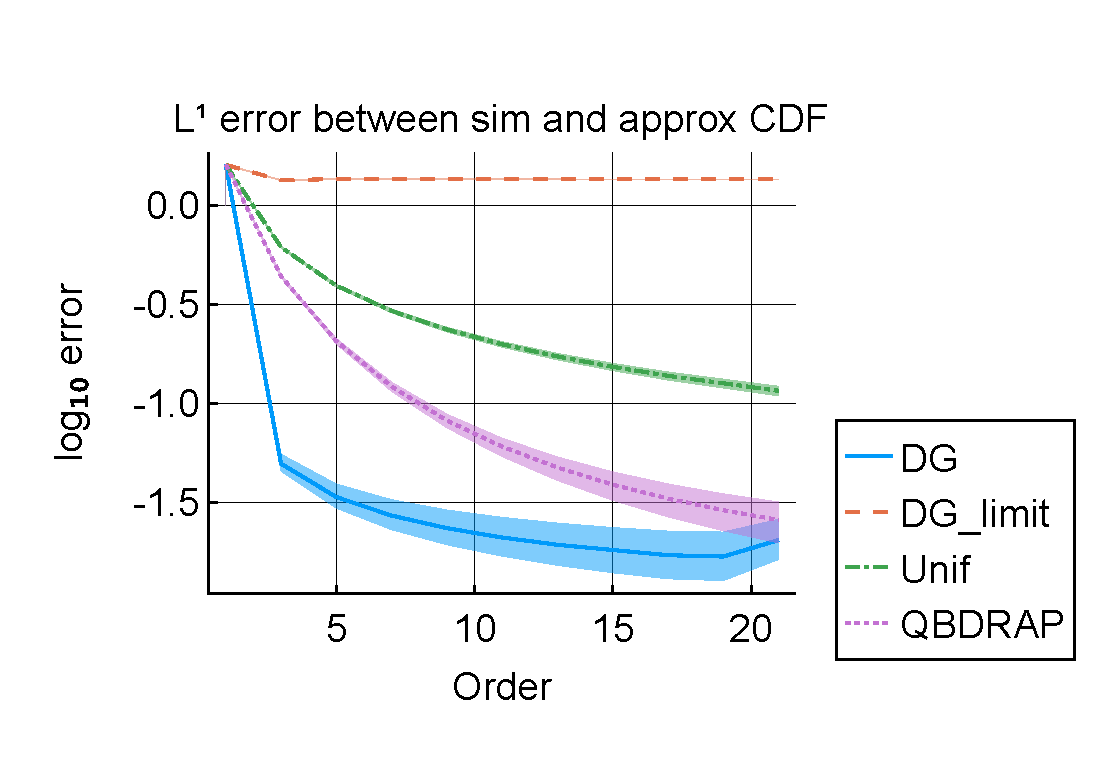
\includegraphics[width=0.5\textwidth,trim={0.75cm 0.8cm 0.25cm 1.25cm},clip]{chapter6/figs/hitting_times_model/hitting_times/point_mass/l1_cdf_error_formatted.pdf}
	\caption{KS (left) and \(L^1\) (right) errors between the simulated and approximated first exit time CDFs (Equation~\ref{eqn: hit cdf}) for Model~\ref{model: simple2} with the point mass initial condition. The approximations were obtained via the DG method (blue solid line), DG method with Generalised MUSCL limiter (orange dashed line), uniformisation method (green dashed line) and QBD-RAP method (purple dotted line). Bootstrapped 90\% confidence intervals are shown by the lighter coloured bars surrounding the lines.} 
	\label{fig: hitting time pm} 
\end{figure}
\begin{figure}
	\centering
	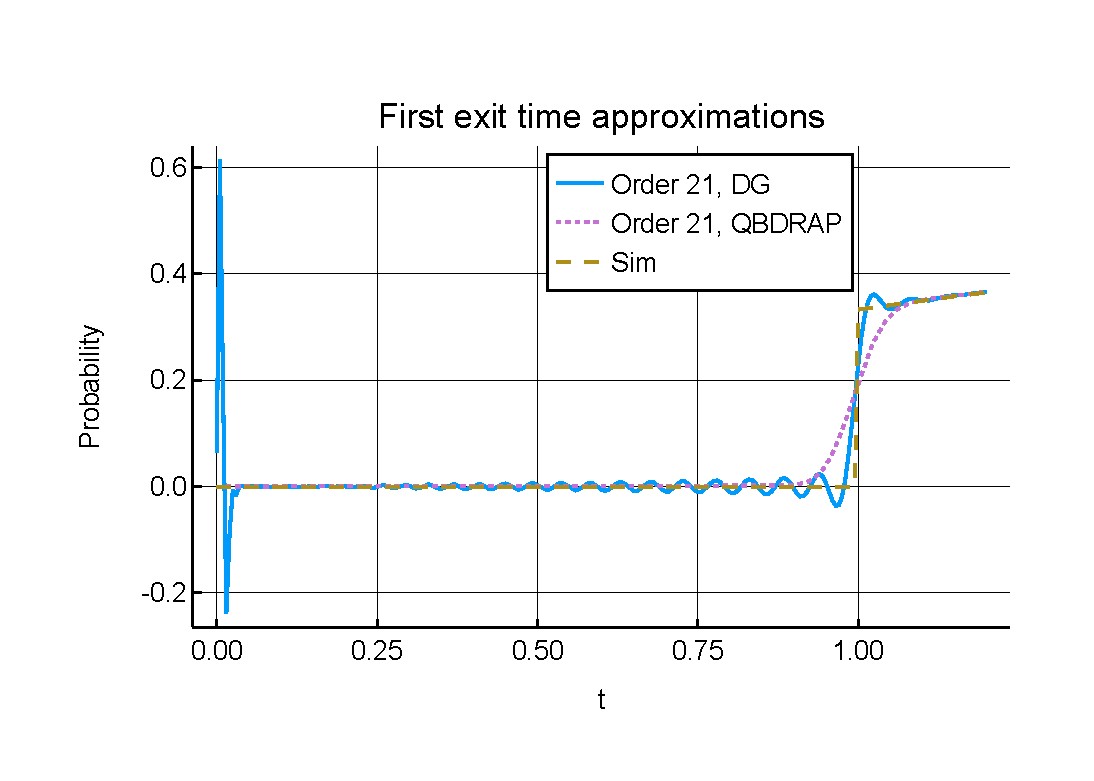
\includegraphics[width=\textwidth]{chapter6/figs/hitting_times_model/hitting_times/point_mass/cdf_order21DG_and_sims.pdf}%
	\caption{Approximations of the CDF of the first exit time in phase 1 for Model~\ref{model: simple2} with the point mass initial condition. The blue line was obtained from the order-21 DG scheme, the purple dotted line from the order-21 QBD-RAP scheme, and the gold dashed line is the empirical CDF obtained via simulation. The DG scheme displays oscillations. } 
	\label{fig: hitting time oscillation} 
\end{figure}

\section{First-return times of fluid-fluid queues}
Here we approximate a model considered in \cite{blnos2022} which is a modified version of a model first presented in \cite{lnp13}. 
\begin{model}\label{model: ffq}
	Consider a stochastic fluid-fluid queue $\{(X(t),Y(t),\varphi(t))\}_{t\geq0},$ where $\{X(t)\}$ and $\{Y(t)\}$ represent the workloads in Buffers~1 and~2 at time $t \geq 0$, respectively, both driven by the phase $\{\varphi(t)\},$ which is a Markov chain on the state space $\mathcal{S} = \{11,10,01,00\}$. Both $\{X(t)\}$ and $\{Y(t)\}$ have a regulated boundary at 0. Here, the state $11$ indicates inputs to both buffers being \textsc{on}, the state $00$ indicates both being \textsc{off}, the state $10$ is when only the first input is \textsc{on}, and the state $01$ is when only the second is \textsc{on}. The input of Buffer~$k$ is switched from \textsc{on} to \textsc{off} with rate $\gamma_k$, and from \textsc{off} to \textsc{on} with rate $\beta_k$, for $k = 1, 2$. Thus, the infinitesimal generator $T$ for $\varphi(t)$ is given by 
	\begin{align*} 
		T = \left[ \begin{array}{cccc} -(\gamma_1 + \gamma_2) & \gamma_2 & \gamma_1 & 0 \\
							\beta_2 & -(\gamma_1 + \beta_2) & 0 & \gamma_1 \\
							\beta_1 & 0 & -(\gamma_2 + \beta_1) & \gamma_2 \\
							0 & \beta_1 &\beta_2 &-(\beta_1 + \beta_2)
	\end{array}\right].
	\end{align*} 

	The net rates of change for $X(t)$, denoted $c_i$, are given by 
	% 
	\begin{align*} 
	& (c_{11},c_{10},c_{01},c_{00})   =  \begin{array}{rrrr} 
	(\lambda_1-\theta_1,  & \lambda_1 -\theta_1, &  -\theta_1, & -\theta_1),
	\end{array}  
	\end{align*} 
	% 
	and the net rates of change for $Y(t)$, denoted $r_i$, are as follows  
	%  
	\begin{align*} 
	(r_{11},r_{10},r_{01},r_{00})  & = \left\{ \begin{array}{lrrrll}  
	% (\lambda_2 -\kappa, & \;\;\;\;0, & \lambda_2 - \kappa, &  \;\;\;\;0) & \text{if } X_t = 0,  Y_t = 0,\\
	%  \vspace*{-0.3cm} \\
												(\lambda_2 - \kappa, & \;\;\;-\kappa,  & \lambda_2 - \kappa, & -\kappa) &\text{if } X_t = 0, \\
												\vspace*{-0.3cm} \\
	%	(\lambda_2 -\theta_2,  &  0,  & \lambda_2 - \theta_2,  & \;\;\;\; 0) & \text{if } X_t \in (0,x^*), Y_t = 0,\\
	%											  \vspace*{-0.3cm} \\
		(\lambda_2 - \theta_2, & -\theta_2, & \lambda_2 - \theta_2, & -\theta_2) & \text{if } X_t \in (0,x^*),\\
												\vspace*{-0.3cm} \\
		(\;\;\;\;\;\;\; \lambda_2, & \;\;\;\;0, & \lambda_2, &  \;\;\;\;0) & \text{if } X_t \geq x^*. \end{array}
												\right.
	\end{align*} 

	For our numerical experiments, we use the parameter choices given in~\citep{lnp13}: 
	% 
		\begin{align} 
			\label{eqn:parameters}
		\gamma_1 & =11, \quad  \beta_1 = 1, \quad \lambda_1 = 12.48, \quad  \theta_1 = 1.6, \quad  \kappa = 2.6, \\
			\label{eqn:parameters-2}
		\gamma_2 & = 22, \quad \beta_2  = 1, \quad  \lambda_2 = 16.25, \quad \theta_2 = 1.0, \quad x^* = 1.6.
		\end{align} 
\end{model}
	
While the true problem has an unbounded domain $[0,\infty)$, the approximations require the domain of approximation to be a finite interval. Here we choose an upper bound of \(48\) and place a regulated boundary at the upper boundary. The effect of this truncation can be partly quantified by evaluating \(\lim\limits_{t\to\infty}\mathbb P\left(X(t) > 48\right)\approx 5.83 \times 10^{-9}\), \(i\in\calS\). 

We obtained approximations to the infinitesimal generator of the fluid queue \(\{(X(t),\varphi(t))\}_{t\geq 0}\) via the DG method, QBD-RAP method and uniformisation method, all of which used a cell width of \(\Delta=0.4\). The matrix resulting from the approximation is then used to approximate the first-return operator \(\Psi(s)\) as discussed in Section~\ref{SOME INTRO SECTION}. Due to the stochastic interpretation of the uniformisation and QBD-RAP schemes, the approximations to \(\Psi(s)\) have a stochastic interpretation as the first-return probabilities of a fluid queue driven by a CTMC and QBD-RAP, respectively. For the DG method the approximation of \(\Psi(s)\) is not well-understood. However, I believe that the resulting operator is a projection operator which, given an initial distribution, projects the distribution of \(X(\theta_2)\) on to a set of polynomial basis functions, much like the DG method itself. 

Ultimately, we want to approximate the first-return distribution 
\begin{align}\label{eqn: first return Y 1}
	\mathbb P(X(\theta_2)\leq x, \varphi(\theta_2)=i\mid \bs X(0)\sim \mu).
\end{align}
For Model~\ref{model: ffq}, it is only possible for the process \(Y(t)\) to return to \(0\) at time \(t\) when \((X(t),\varphi(t))\in[0,1.6)\times \{10,00\}\). As such, evaluate the approximations over this region only. We use a grid of 10,001 points at which to evaluate the approximations of the CDF in each phase. We consider first the initial distribution which is a point mass at \(Y(0)=0,\, X(0)=5,\, \varphi(0)=01\). 

For comparison, we simulated 5,000,000 realisations of the fluid-fluid queue and recorded the value of \(X\) and \(\varphi\) at the time of first return of the second fluid, \(Y\). The empirical approximation of (\ref{eqn: first return Y 1}) was then constructed, and error metrics for the difference between the empirical CDF and the approximations was computed. To account for Monte-Carlo errors, we used a bootstrap with 1,000 bootstrap samples to construct 1,000 bootstrap samples of the error estimates and recorded the 5th and 95th percentiles of the error distribution. Each of the 1,000 bootstrap samples was constructed by resampling the original 5,000,000 realisations 5,000,000 times, with replacement.

In Figure~\ref{fig: ffq return cts} we plot the error metrics for the approximations to the distribution (\ref{eqn: first return Y 1}). The DG method performs best converging rapidly until the error in the approximation scheme is swamped by other numerical errors. Here, the first return distribution appears to be smooth, hence we might expect the DG method to perform well. Note that there is a significant number other sources of error here; machine precision errors, errors in solving the Ricatti equation to approximate \(\Psi(s)\), errors from approximating error metrics (numerical integration/finding KS statistic), and truncation errors. Furthermore, for the QBD-RAP, since the parameters \(\bs \alpha,\,\bs S,\,\bs s\,\) and \(\bs D\) are found numerically, then there is another source of error from this. 

Figure~\ref{fig: ffq return cts} also shows that the uniformisation and QBD-RAP methods also appear to be converging, albeit, at a slower rate. 
\begin{figure}
	\centering
	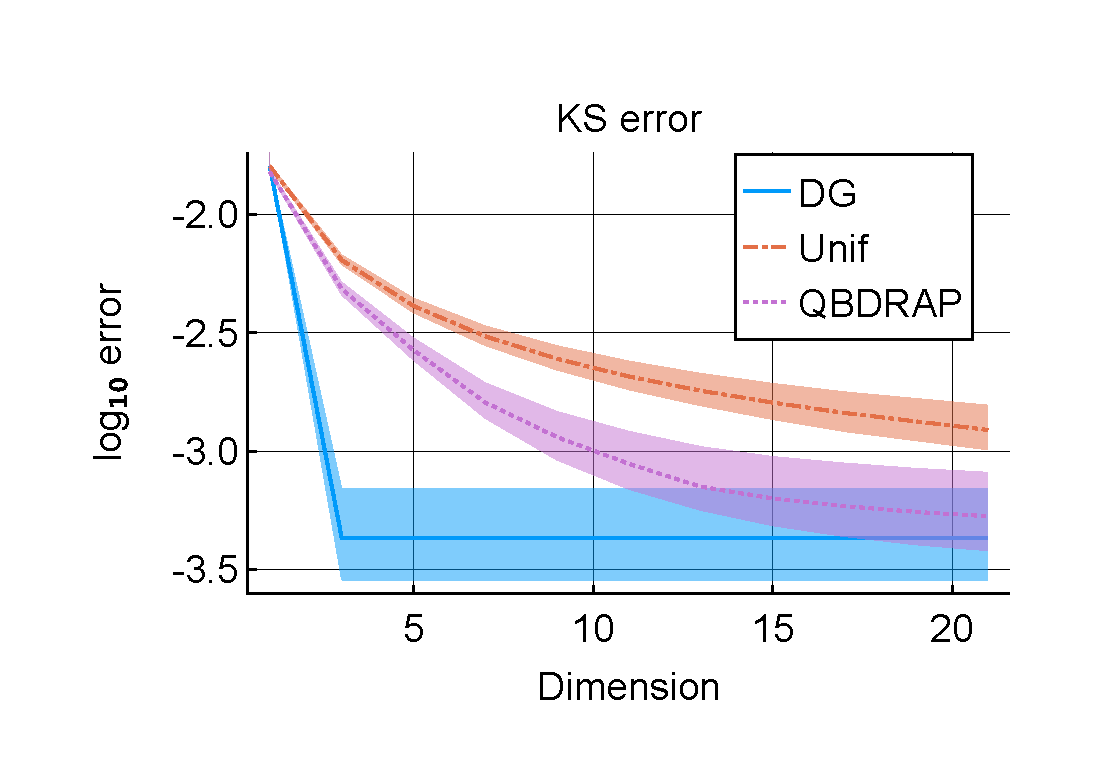
\includegraphics[width=0.5\textwidth,trim={0.75cm 0.8cm 0.25cm 1.25cm},clip]{chapter6/figs/ffq/cts/ks_error_formatted.pdf}%
	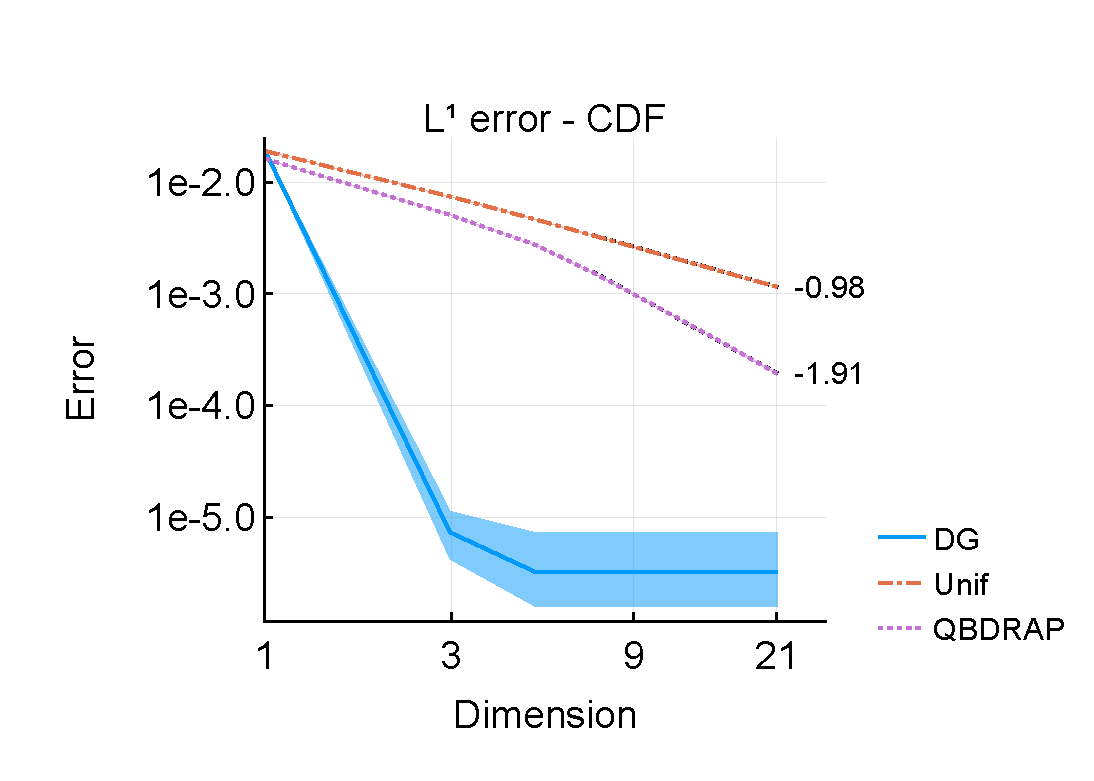
\includegraphics[width=0.5\textwidth,trim={0.75cm 0.8cm 0.25cm 1.25cm},clip]{chapter6/figs/ffq/cts/l1_cdf_error_formatted.pdf}
	\caption{KS (left) and \(L^1\) (right) errors between the simulated and approximated CDFs of \(X(\theta_2)\) (Equation~\ref{eqn: first return Y 1}) for Model~\ref{model: ffq}. The approximations were obtained via the DG method (blue solid line), uniformisation method (green dashed line) and QBD-RAP method (purple dotted line). Bootstrapped 90\% confidence intervals are shown by the lighter coloured bars surrounding the lines.} 
	\label{fig: ffq return cts} 
\end{figure}

By modifying slightly Model~\ref{model: ffq}, we can construct a first return distribution which is discontinuous. 
\begin{model}\label{model: ffq2}
	Consider a fluid-fluid queue which is the same as Model~\ref{model: ffq} except 
	\begin{align}
		r_{00}(X(t)) = \begin{cases}
			-\kappa, & \mbox{ if }X(t)=0,\\
			-\theta_2, & \mbox{ if }X(t)=\in(0,x^*),\\
			\theta_2, & \mbox{ if }X(t)\geq x^*.
		\end{cases}
	\end{align}
	Further, consider the initial distribution which is a point-mass at \(Y(0)=0,\, X(0)=2, \varphi(0)=00\).
\end{model}
As before, we use the DG, uniformisation and QBD-RAP methods to approximate the model, and compare to simulations. 

For Model~\ref{model: ffq2} there is a point mass at \(X(\theta_2)=1.2\) of magnitude \(e^{-(\beta_1+\beta_2)}\times 0.5\), which occurs when the phase remains \(\varphi(t)=00\) until this \(\theta_2\).

Figure~\ref{fig: ffq return discts} plots the error metrics for the first return distribution. Observing Figure~\ref{fig: ffq return discts} we see that the DG method performs well, followed by the QBD-RAP method, then the uniformisation method performs worst. However, the DG method results in an oscillatory solution with the CDF taking impossible values (decreasing at points) as shown in Figure~\ref{fig: ffq2 oscillation}
\begin{figure}
	\centering
	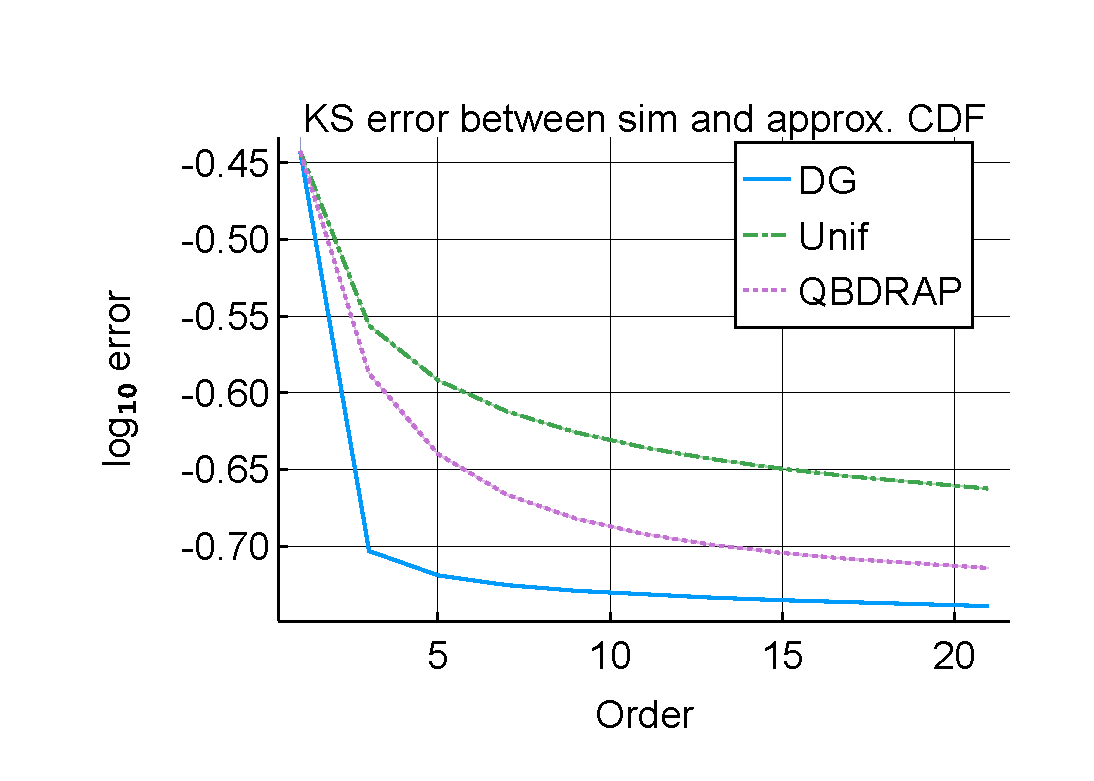
\includegraphics[width=0.5\textwidth,trim={0.75cm 0.8cm 0.25cm 1.25cm},clip]{chapter6/figs/ffq/discts/ks_error_formatted.pdf}%
	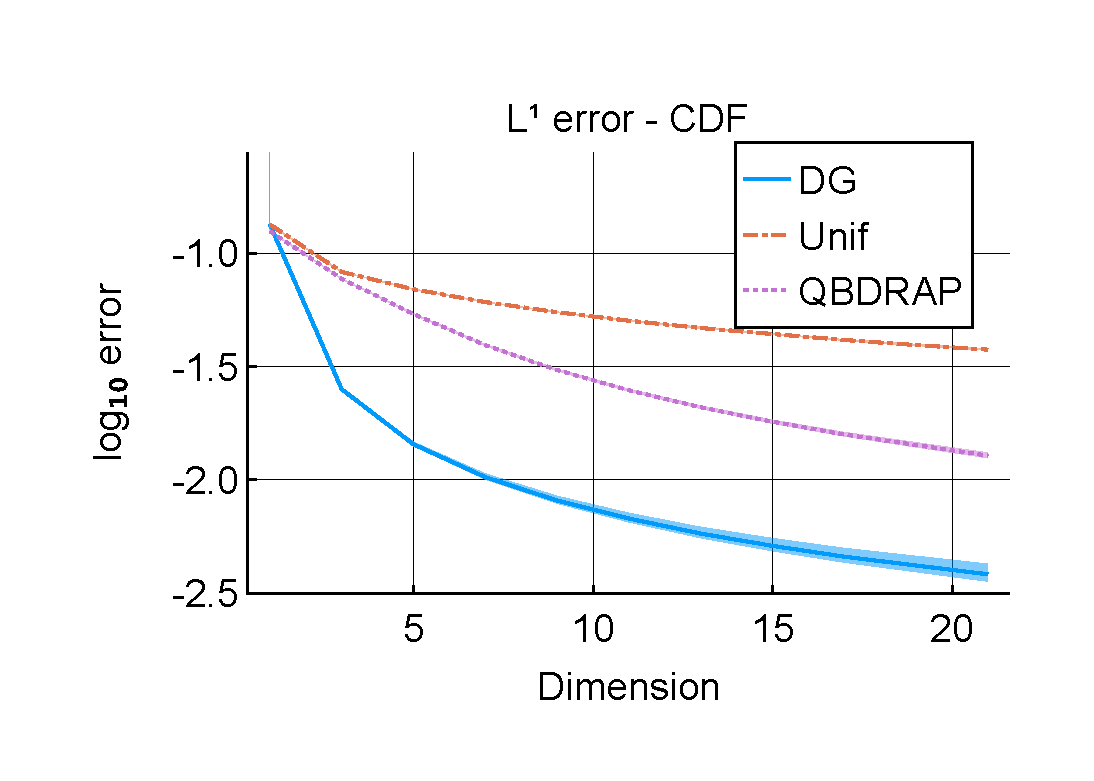
\includegraphics[width=0.5\textwidth,trim={0.75cm 0.8cm 0.25cm 1.25cm},clip]{chapter6/figs/ffq/discts/l1_cdf_error_formatted.pdf}
	\caption{KS (left) and \(L^1\) (right) errors between the simulated and approximated CDFs of \(X(\theta_2)\) (Equation~\ref{eqn: first return Y 1}) for Model~\ref{model: ffq2}. The approximations were obtained via the DG method (blue solid line), uniformisation method (green dashed line) and QBD-RAP method (purple dotted line). Bootstrapped 90\% confidence intervals are shown by the lighter coloured bars surrounding the lines.} 
	\label{fig: ffq return discts} 
\end{figure}
\begin{figure}
	\centering
	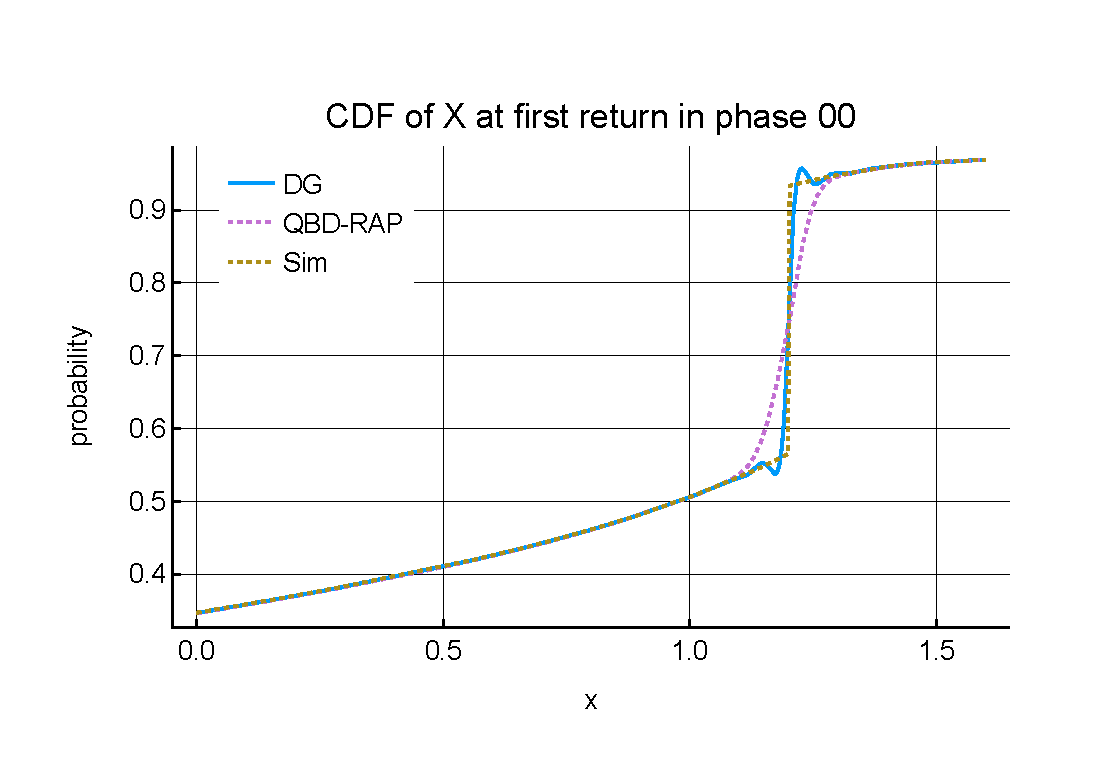
\includegraphics[width=\textwidth]{chapter6/figs/ffq/discts/phase_4_cdf.pdf}%
	\caption{Approximations of the CDF of the first exit time in phase 1 for Model~\ref{model: simple2} with the point mass initial condition. The blue line was obtained from the order-21 DG scheme, the purple dotted line from the order-21 QBD-RAP scheme, and the gold dashed line is the empirical CDF obtained via simulation. The DG scheme displays oscillations. } 
	\label{fig: ffq2 oscillation} 
\end{figure}

\FloatBarrier
\section{Discussion}
In this chapter we have numerically investigated some properties of the QBD-RAP approximation scheme and compared it to existing methods; the uniformisation scheme of \cite{bo2013} and the discontinuous Galerkin scheme. In general, the numerical experiments show that, for problems with discontinuities, the DG approximation can exhibit oscillations and negativity, while the QBD-RAP and uniformisation approximations avoid this and, of the latter two, the QBD-RAP scheme often converges faster. To avoid the problems of oscillations and negativity, we can sometimes employ a \emph{slope limiter} with the DG scheme, which effectively reduces the scheme to linear in the regions where oscillations are detected. The numerical experiments demonstrate the loss of accuracy in the approximation when a slope limiter is used for a discontinuous problem. Moreover, for the application of the methods to fluid-fluid queues, there is no useful way to apply the concept of a slope limiter. %When the slope limiter detects oscillations in the approximate solution, it reduces the DG scheme to linear in the region surrounding the oscillations, otherwise, the slope limiter leaves the solution unchanged. Thus, the slope limiter permits high-order approximations away from oscillations, while also removing oscillations. 
In general, we observe that the smoother the problem the better the performance of the DG method, and it rapidly surpasses the performance of the other two methods. For smooth problems the DG method is almost unbeatable. 

As a first step in the numerical experiments, we examined the ability for each method to approximate different initial conditions. For the DG method, this is equivalent to a projection of the initial condition on to a set of basis polynomials. For the uniformisation method this is equivalent to projecting the initial condition on to a basis of constant functions. Section~\ref{sec: comp} demonstrates that the DG (projection) scheme can result in oscillations and negative regions in the approximation when the initial condition is discontinuous. The uniformisation and QBD-RAP methods avoid this problem, but appear to have higher errors and the QBD-RAP method appears to have the largest errors. For discontinuous initial conditions the rates of convergence are comparable for all three methods. However, when the initial condition to be approximated is sufficiently smooth, then the DG approximation is \emph{far} superior. 

Next, we instrumented the performance of approximations for a simple travelling wave problem with various initial conditions. For this problem the solution is given in terms of the initial condition by \(f(x,t) = f(x-t,0)\). Once again, for discontinuous problems, the DG method can display oscillations and negativity, while the other methods (DG with slope limiter, uniformisation and QBD-RAP methods) avoid this. Further, for discontinuous problems the rates of convergence of the QBD-RAP and DG methods can be similar. For smooth problems the DG method is superior. 

We then instrument the performance of the approximations on a simple fluid queue. We first look at the stationary distribution, which is known to be smooth. Since the problem is smooth, then the DG method is superior as expected. Of the uniformisation and QBD-RAP methods, the QBD-RAP method gives more accurate solutions. We then turn our attention to approximating transient distributions for the same models and consider two different initial conditions, a point-mass and an exponential initial condition. The discontinuous initial condition results in a discontinuous transient distribution. As for the exponential initial condition, this example demonstrates that, even if the initial condition appears `nice', it can still result in discontinuous, or non-differetiable solutions. The numerical evidence suggests that the DG method can display oscillations, while the other methods do not. The DG method with slope limiter detects the oscillations and reduces the method to linear. Of the uniformisation and QBD-RAP methods, the latter performs better. 

Next we look at exit times for the same fluid queue with two initial conditions, an exponential initial condition and a point-mass. We look at the exit time of the fluid level from the interval \((0,1)\). For this problem there is never any in-flow of mass at the boundaries of the interval and so, for a solution to be continuous, the initial condition needs to be chosen carefully, otherwise discontinuities in the \textit{transient distribution} may result, as is the case for both initial conditions here. The numerical results suggest that, due to the discontinuities in the problems, the DG method can perform not as well as we might expect. Since the uniformisation and QBD-RAP methods can handle discontinuities, they perform as expected, with the QBD-RAP method performing better than the uniformisation. 

Lastly, we apply the DG, uniformisation and QBD-RAP methods to some simple fluid-fluid queues. In the first example, which appears to have a smooth solution, the DG method performs very well. Of the other two methods the QBD-RAP method performs better than the uniformisation. In the second example, which has a discontinuity, the DG method produces the lowest errors, but exhibits oscillations in the solution. The other two methods do not produce oscillations, and of the two the QBD-RAP method performs best. 

In conclusion, when the problem is known to be smooth, the DG method is very likely to produce excellent results. However, for discontinuous problems, the method can show oscillations and infeasible or negative regions of the solution. The slope limiter overcomes this, but reduces the accuracy of the DG method to linear near discontinuities, sometimes severely affecting the quality of the approximation. The uniformisation and QBD-RAP methods are alternative approximation schemes which exhibit larger errors, but avoid oscillatory solutions and ensure positivity. Of uniformisation and QBD-RAP methods, the latter seems to produce lower errors. 
